\documentclass[10pt, twocolumn, letterpaper]{article}

%% ── Tipografía Times New Roman ──────────────────────────────
\usepackage{mathptmx}
\usepackage[T1]{fontenc}
\usepackage[utf8]{inputenc}
\usepackage{textcomp}

%% ── Idiomas (español principal, inglés y portugués para resumen) ──
\usepackage[portuguese,english,spanish,es-noshorthands]{babel}

%% ── Matemáticas (ecuaciones alineadas a la izquierda) ───────
\usepackage[fleqn]{amsmath}
\usepackage{amssymb}
\setlength{\mathindent}{0pt}

%% ── Diseño de página (Letter, márgenes 16,9 mm, col. 4,3 mm) ──
\usepackage{geometry}
\geometry{
  letterpaper,
  top    = 16.9mm,
  bottom = 16.9mm,
  left   = 16.9mm,
  right  = 16.9mm,
  columnsep = 4.3mm
}

%% ── Interlineado 1,05 y párrafos sin espacio extra ──────────
\usepackage{setspace}
\setstretch{1.05}
\setlength{\parindent}{12pt}
\setlength{\parskip}{0pt}

%% ── Secciones en versalita + numeración romana ───────────────
\usepackage{titlesec}
\renewcommand{\thesection}{\Roman{section}}
\renewcommand{\thesubsection}{\Alph{subsection}}
\titleformat{\section}
  {\normalfont\normalsize\scshape\centering}{\thesection.}{0.5em}{}
\titleformat{\subsection}
  {\normalfont\normalsize\itshape}{\thesubsection.}{0.5em}{}
\titlespacing{\section}{0pt}{6pt plus 2pt}{3pt}
\titlespacing{\subsection}{0pt}{4pt plus 2pt}{2pt}

%% ── Capitular (primera letra de la Introducción) ─────────────
\usepackage{lettrine}

%% ── Figuras, tablas y flotantes ─────────────────────────────
\usepackage{graphicx}
\usepackage{booktabs}
\usepackage{float}
\usepackage{subcaption}
\usepackage{caption}
\usepackage{siunitx}
\sisetup{output-decimal-marker={,}, group-separator={\,}}

\renewcommand{\thetable}{\Roman{table}}

\captionsetup[figure]{
  font          = footnotesize,
  labelsep      = period,
  justification = justified,
  singlelinecheck = false,
  name          = Fig.
}
\captionsetup[table]{
  font            = footnotesize,
  labelfont       = sc,
  labelsep        = newline,
  justification   = centering,
  singlelinecheck = false,
  name            = Tabla,
  position        = above
}

%% ── Hipervínculos ────────────────────────────────────────────
\usepackage{xcolor}
\usepackage{hyperref}
\hypersetup{
  colorlinks = true,
  linkcolor  = black,
  citecolor  = black,
  urlcolor   = black
}

%% ── Bibliografía IEEE numerada por orden de aparición ────────
\usepackage[numbers,sort&compress]{natbib}
\renewcommand{\refname}{Referencias}
\renewcommand{\bibfont}{\footnotesize}

%% ── Microtipografía ─────────────────────────────────────────
\usepackage{microtype}

%% ── Título ───────────────────────────────────────────────────
\title{%
  {\fontsize{18}{22}\selectfont\textbf{%
    Análisis espacial de la susceptibilidad a los movimientos en masa
    mediante Proceso de Poisson No Homogéneo: aplicación en Medellín, Colombia}}%
  \\[6pt]%
  {\fontsize{18}{22}\selectfont\textbf{\textit{%
    Spatial Analysis of Landslide Susceptibility Using a Non-Homogeneous
    Poisson Process: Application in Medellín, Colombia}}}%
}

%% ── Autor ────────────────────────────────────────────────────
\author{%
  {\fontsize{11}{13}\selectfont E.~Aristizábal}%
  \thanks{\footnotesize
        Este trabajo se deriva del proyecto Geohazards, adscrito al
    Departamento de Geociencias y Medio Ambiente, Facultad de Minas,
    Universidad Nacional de Colombia, Sede Medellín, Colombia.
    Grupo de Investigación en Geología Ambiental (GEA).\\[2pt]
    \hspace*{12pt}E.~Aristizábal, Departamento de Geociencias y Medio Ambiente,
    Facultad de Minas, Universidad Nacional de Colombia, Sede Medellín,
    Medellín, Colombia. Correo:
    \href{mailto:evaristizabalg@unal.edu.co}{evaristizabalg@unal.edu.co}.}%
}
\date{}

% ─────────────────────────────────────────────────────────────
\begin{document}

%% Título + resúmenes en ancho completo (una sola columna)
\twocolumn[{%
  \maketitle
  \vspace{-4pt}
  \noindent\rule{\linewidth}{0.4pt}\vspace{3pt}
  {\small\noindent
    \textbf{\textit{Resumen}}\textemdash\textbf{Los movimientos en masa
    representan una de las amenazas naturales más destructivas en regiones
    montañosas tropicales densamente urbanizadas. La modelación estadística
    de la susceptibilidad ha recurrido históricamente a enfoques de regresión
    logística o aprendizaje automático que tratan el inventario como una
    respuesta binaria de presencia-ausencia en una cuadrícula regular,
    ignorando la naturaleza de proceso puntual de los datos. Este estudio
    aplica un Proceso de Poisson No Homogéneo (NHPP) mediante la aproximación
    INLA a un inventario de \num{2504} movimientos en masa en Medellín
    (Colombia). La log-intensidad se modela como función log-lineal de cuatro
    predictores derivados de un Modelo Digital de Elevación de \SI{2}{m}:
    pendiente, aspecto, indicador de suelos finos y cobertura urbana. El
    modelo produce estimaciones identificables y físicamente interpretables:
    pendiente (0,901; IC 95\,\%: [0,856;\,0,946]),
    aspecto (\textminus0,243; [\textminus0,283;\,\textminus0,204]),
    cobertura urbana (\textminus0,971; [\textminus1,154;\,\textminus0,788]) y
    suelos finos (\textminus0,709; [\textminus0,790;\,\textminus0,628]),
    confirmando el control geomorfológico y litológico de la susceptibilidad.
    La capacidad discriminativa del modelo es AUC~=~0,762, superior a modelos de
    proceso puntual topográficos reportados en la literatura para contextos similares.
    El enfoque ofrece una base probabilística rigurosa para la evaluación
    cuantitativa de la amenaza por movimientos en masa.}\\[3pt]
    %
    \textbf{\textit{Palabras clave}}\textemdash\textbf{Medellín; movimientos
    en masa; Proceso de Poisson No Homogéneo; proceso puntual espacial;
    susceptibilidad.}\\[3pt]
    %
    \foreignlanguage{english}{%
    \textbf{\textit{Abstract}}\textemdash\textbf{Landslides represent one of
    the most destructive natural hazards in densely urbanized tropical
    mountainous regions. Statistical susceptibility modeling has historically
    relied on logistic regression or machine learning approaches that treat
    the inventory as a binary presence-absence response on a regular grid,
    ignoring the point process nature of the data. This study applies a
    Non-Homogeneous Poisson Process (NHPP) through the INLA approximation
    to an inventory of \num{2504} landslides in Medellín, Colombia. The
    log-intensity is modeled as a log-linear function of four predictors
    derived from a \SI{2}{m} resolution Digital Elevation Model: slope,
    aspect, fine-soil indicator, and urban cover. The model produces
    identifiable and physically interpretable estimates: slope
    (0.901; 95\,\% CI: [0.856;\,0.946]), aspect
    (\textminus0.243; [\textminus0.283;\,\textminus0.204]), urban cover
    (\textminus0.971; [\textminus1.154;\,\textminus0.788]), and fine soils
    (\textminus0.709; [\textminus0.790;\,\textminus0.628]), confirming the
    geomorphological and lithological control of susceptibility. The
    discriminative capacity of the model is AUC~=~0.762, superior to
    topographic point process models reported in the literature for similar
    contexts. The approach offers a rigorous probabilistic basis for
    quantitative landslide hazard assessment.}\\[3pt]
    %
    \textbf{\textit{Keywords}}\textemdash\textbf{landslide susceptibility;
    Medellín; Non-Homogeneous Poisson Process; spatial point process.}}\\[3pt]
    %
    \foreignlanguage{portuguese}{%
    \textbf{\textit{Resumo}}\textemdash\textbf{Os movimentos de massa
    representam uma das ameaças naturais mais destrutivas em regiões
    montanhosas tropicais densamente urbanizadas. A modelagem estatística
    da suscetibilidade tem recorrido historicamente a abordagens de
    regressão logística ou aprendizado de máquina que tratam o inventário
    como uma resposta binária de presença-ausência em uma grade regular,
    ignorando a natureza de processo pontual dos dados. Este estudo aplica
    um Processo de Poisson Não Homogêneo (PPNH) mediante a aproximação INLA
    a um inventário de \num{2504} movimentos de massa em Medellín, Colômbia.
    A log-intensidade é modelada como função log-linear de quatro preditores
    derivados de um Modelo Digital de Elevação de \SI{2}{m} de resolução:
    declividade, aspecto, indicador de solos finos e cobertura urbana. O
    modelo produz estimativas identificáveis e fisicamente interpretáveis,
    confirmando o controle geomorfológico e litológico da suscetibilidade.
    A capacidade discriminativa do modelo é AUC~=~0,762, superior a
    modelos de processo pontual topográficos reportados na literatura para
    contextos similares. A abordagem oferece uma base probabilística rigorosa
    para a avaliação quantitativa da ameaça por movimentos de massa.}\\[3pt]
    %
    \textbf{\textit{Palavras-chave}}\textemdash\textbf{Medellín; movimentos
    de massa; Processo de Poisson Não Homogêneo; processo pontual espacial;
    suscetibilidade.}}%
  }% cierra {\small\noindent
  \vspace{3pt}
  \noindent\rule{\linewidth}{0.4pt}
  \vspace{8pt}
}]

% ─────────────────────────────────────────────────────────────
\section{Introducción}
\label{sec:intro}
% ─────────────────────────────────────────────────────────────

\lettrine[lines=2]{L}{a} modelación de la susceptibilidad por movimientos en
masa ha evolucionado desde métodos heurísticos basados en criterios de expertos
hasta modelos estadísticos y de aprendizaje automático \cite{reichenbach2018}. La mayoría de
estos métodos estadísticos proyectan el inventario de eventos sobre una
cuadrícula regular de celdas, asignan etiquetas binarias de presencia-ausencia
de movimientos en masa y modelan la probabilidad de ocurrencia en función de
atributos como la pendiente, la curvatura, la litología o el uso del suelo,
entre otros \cite{guzzetti2005, lombardo2018}. Aunque operativamente
conveniente, esta discretización conlleva pérdidas de información espacial
importantes y confunde la ausencia verdadera de ocurrencia de movimientos en
masa con la falta de observación o registro en el inventario, lo que sesga la
evaluación de la susceptibilidad \cite{lombardo2018}.

En las últimas décadas, los modelos de aprendizaje automático han alcanzado niveles de desempeño predictivo
excepcionalmente altos en la evaluación de la susceptibilidad por movimientos en
masa, con valores de Área Bajo la Curva (AUC [0--1]) que frecuentemente superan
0,90 en conjuntos de validación \cite{reichenbach2018}. Sin embargo, estos
modelos operan esencialmente como \emph{cajas negras}: su arquitectura interna
impide la interpretación directa de las relaciones entre covariables y respuesta
en términos del proceso físico subyacente, dificultando la validación científica
de los resultados y la transferencia del conocimiento entre contextos
geomorfológicos \cite{lombardo2018}. Esta limitación es particularmente
relevante en el ámbito de los movimientos en masa, donde la identificación
cuantitativa de los factores de control ---topografía, litología, uso del
suelo--- tiene implicaciones directas para la gestión del riesgo y el diseño de
medidas de reducción de la amenaza.

Los modelos de la familia de los Modelos Lineales Generalizados (GLM), en
cambio, vinculan cada predictor a la respuesta mediante coeficientes
interpretables que cuantifican el efecto de cada variable,
permitiendo conectar los resultados estadísticos con el conocimiento
geomorfológico del proceso. En particular, el GLM de Poisson
modela el número esperado de eventos en cada unidad espacial de análisis
(celda, unidad de ladera, cuenca, etc.) como función log-lineal de las
covariables, lo que constituye la forma discreta, denominada \emph{modelo
espacial de área}, de un mecanismo generador más fundamental. En el modelo de
área, la autocorrelación espacial entre unidades contiguas puede incorporarse mediante componentes
autorregresivos condicionales (CAR) \cite{besag1974, besag1991}, dando lugar a
modelos lineales generalizados jerárquicos de Poisson con estructura espacial.
Este paradigma opera en el espacio discreto: la susceptibilidad se expresa como
función constante por partes que cambia abruptamente en los límites de los
polígonos, y los resultados pueden depender del tamaño y la forma de las
unidades elegidas, el Problema de la Unidad de Área Modificable
(MAUP) \cite{openshaw1984, fotheringham1991}.

Cuando, en cambio, el inventario se concibe como una nube de puntos en el
espacio continuo $\mathbb{R}^2$, esta misma estructura conduce de manera
natural al marco de los \emph{procesos puntuales espaciales}, donde la función
de intensidad $\lambda(\mathbf{s})$ varía de forma continua y suave en todo el
dominio sin imponer unidades de agregación predefinidas. Desde esta perspectiva,
el inventario de movimientos en masa es mejor entendido como una realización de
un conjunto aleatorio de puntos en el dominio continuo
$\Omega \subset \mathbb{R}^2$, y la inferencia estadística apunta a la función
de intensidad espacialmente variable $\lambda(\mathbf{s})$ que gobierna el
número esperado de eventos por unidad de área \cite{diggle2013}. El modelo más
parsimonioso de esta familia es el \emph{Proceso de Poisson No Homogéneo}
(NHPP): los eventos son condicionalmente independientes dado
$\lambda(\mathbf{s})$, y esta intensidad se modela como función log-lineal de
las covariables espaciales, la misma estructura del GLM de Poisson, pero
formulada en el dominio continuo sin necesidad de imponer una cuadrícula. Este
enfoque evita la discretización arbitraria en celdas, suprime la ambigüedad de
las ausencias (celdas sin movimientos en masa) y produce una superficie de
susceptibilidad continua directamente interpretable como densidad esperada de
eventos por unidad de área.

La aplicación del proceso puntual espacial a los movimientos en masa sigue
siendo escasa en la literatura. Lombardo et al.\ \cite{lombardo2019}
demostraron el enfoque para flujos de detritos en Sicilia, y
Lombardo et al.\ \cite{lombardo2020} lo extendieron a contextos
espacio-temporales. En el contexto andino, Aristizábal et al.\
\cite{aristizabal2025ag} han aplicado recientemente el modelo de Poisson
espacial de área, con componente CAR sobre unidades de ladera, al departamento
de Antioquia, Colombia; ese enfoque opera en el espacio discreto de los
polígonos. En este trabajo se implementa un proceso puntual espacial en el
dominio continuo, \emph{Proceso de Poisson No Homogéneo} (NHPP), para los
movimientos en masa en la ciudad de Medellín, Colombia, con dos predictores
topográficos y considerando la cobertura urbana/rural y los materiales que
conforman las laderas.

% ─────────────────────────────────────────────────────────────
\section{Área de estudio}
\label{sec:study_area}
% ─────────────────────────────────────────────────────────────

El Valle de Aburrá, donde se encuentra la ciudad de Medellín, es un valle
intramontano de aproximadamente \SI{1165}{km^2} situado en la Cordillera Central
de los Andes colombianos ($6^\circ6'$--$6^\circ41'$\,N,
$75^\circ45'$--$75^\circ21'$\,O). La topografía es característica de los Andes
tropicales: las elevaciones oscilan entre aproximadamente 1300\,m s.n.m.\ en el
fondo del valle y más de 2600\,m en las crestas, con flancos empinados
disectados por numerosas quebradas tributarias del río Medellín
\cite{aristizabal2026}. Geomorfológicamente, el valle está modelado por la
convergencia oblicua de las placas de Nazca y del Caribe con la placa
Sudamericana \cite{trenkamp2002, cediel2003}, que genera un levantamiento
activo, fallas y una topografía altamente montañosa que favorece
intrínsecamente los procesos de remoción en masa \cite{aristizabal2025}. La
región alberga más de 3,6 millones de habitantes, de los cuales el
95\,\% reside en áreas urbanas que ocupan aproximadamente \SI{340}{km^2}; su
crecimiento demográfico fue 30 veces mayor entre 1905 y 2005
\cite{aristizabal2026}. Los movimientos en masa representan la amenaza natural
más recurrente: causan tres de cada diez desastres reportados y el
75\,\% de las víctimas anuales por eventos naturales en la región
\cite{gomez2023}.

El clima es tropical bimodal, regulado principalmente por la migración
meridional de la Zona de Convergencia Intertropical (ZCIT) \cite{bedoya2019,
aristizabal2026, poveda2011}. Las precipitaciones medias anuales oscilan entre
1500 y 2500\,mm, con dos temporadas lluviosas bien definidas: abril--junio
(AMJ) y septiembre--noviembre (SON) \cite{bedoya2019, aristizabal2026}. La
variabilidad interanual está fuertemente modulada por el fenómeno El
Niño-Oscilación del Sur (ENOS): las fases La Niña incrementan
significativamente las precipitaciones ---en particular durante la segunda
temporada lluviosa--- aumentando la humedad del suelo antes del inicio de las
épocas húmedas \cite{aristizabal2026, poveda2011}. La lluvia desencadena el
92\,\% de todos los movimientos en masa registrados en los Andes colombianos
entre 1970 y 2023 \cite{aristizabal2020}.

Los terrenos están conformados predominantemente por rocas metamórficas
---gneis, esquistos y anfibolitas--- que conforman el basamento de la Cordillera
Central \cite{cediel2003}. Localmente se presentan
cuerpos intrusivos granodioríticos y gabros, rocas volcánicas andesíticas a
basálticas intercaladas con depósitos volcanoclásticos, y rocas ultramáficas
(serpentinitas y peridotitas) producto de secuencias ofiolíticas \cite{cediel2003}.
Sobre estas unidades se desarrollan perfiles de meteorización profundos y
heterogéneos: en granitoides, los suelos residuales y saprolitos de color
amarillo-rojizo (Munsell 10YR\,7/4) superan
los 50\,m de espesor;
en rocas ultrabásicas y metamórficas, los perfiles son más delgados
(10--20\,m), de color naranja-rojizo (Munsell 7,5YR\,7/6) y con abundantes
fragmentos muy meteorizados \cite{aristizabal2005, aristizabal2025}. Los
materiales de ladera están dominados por depósitos derivados de procesos de
remoción en masa de largo plazo \cite{aristizabal2005}.

% ─────────────────────────────────────────────────────────────
\section{Datos}
\label{sec:data}
% ─────────────────────────────────────────────────────────────

El inventario de movimientos en masa utilizado comprende \num{2504} eventos
(deslizamientos superficiales, flujos de detritos y deslizamientos
translacionales) compilado mediante interpretación sistemática de imágenes de
satélite de resolución submétrica disponibles en Google Earth entre 2001 y 2024
(Fig.~\ref{fig:inventario}). A diferencia de los inventarios basados en
registros históricos institucionales, que introducen un sesgo de detección
hacia eventos de mayor magnitud o localizados en zonas urbanizadas con mayor
cobertura mediática, el inventario de percepción remota permite detectar
movimientos en masa de forma espacialmente uniforme a lo largo del período de
disponibilidad de imágenes de alta resolución. Esta estrategia de compilación
reduce el sesgo espacial de observación y produce un inventario más
representativo de la distribución de la susceptibilidad. Los eventos están
georeferenciados como localizaciones puntuales de la zona de iniciación. La
densidad media es de aproximadamente 7,08 eventos km$^{-2}$, con agrupamiento
alto en las laderas del valle.

\begin{figure}[htbp]
  \centering
  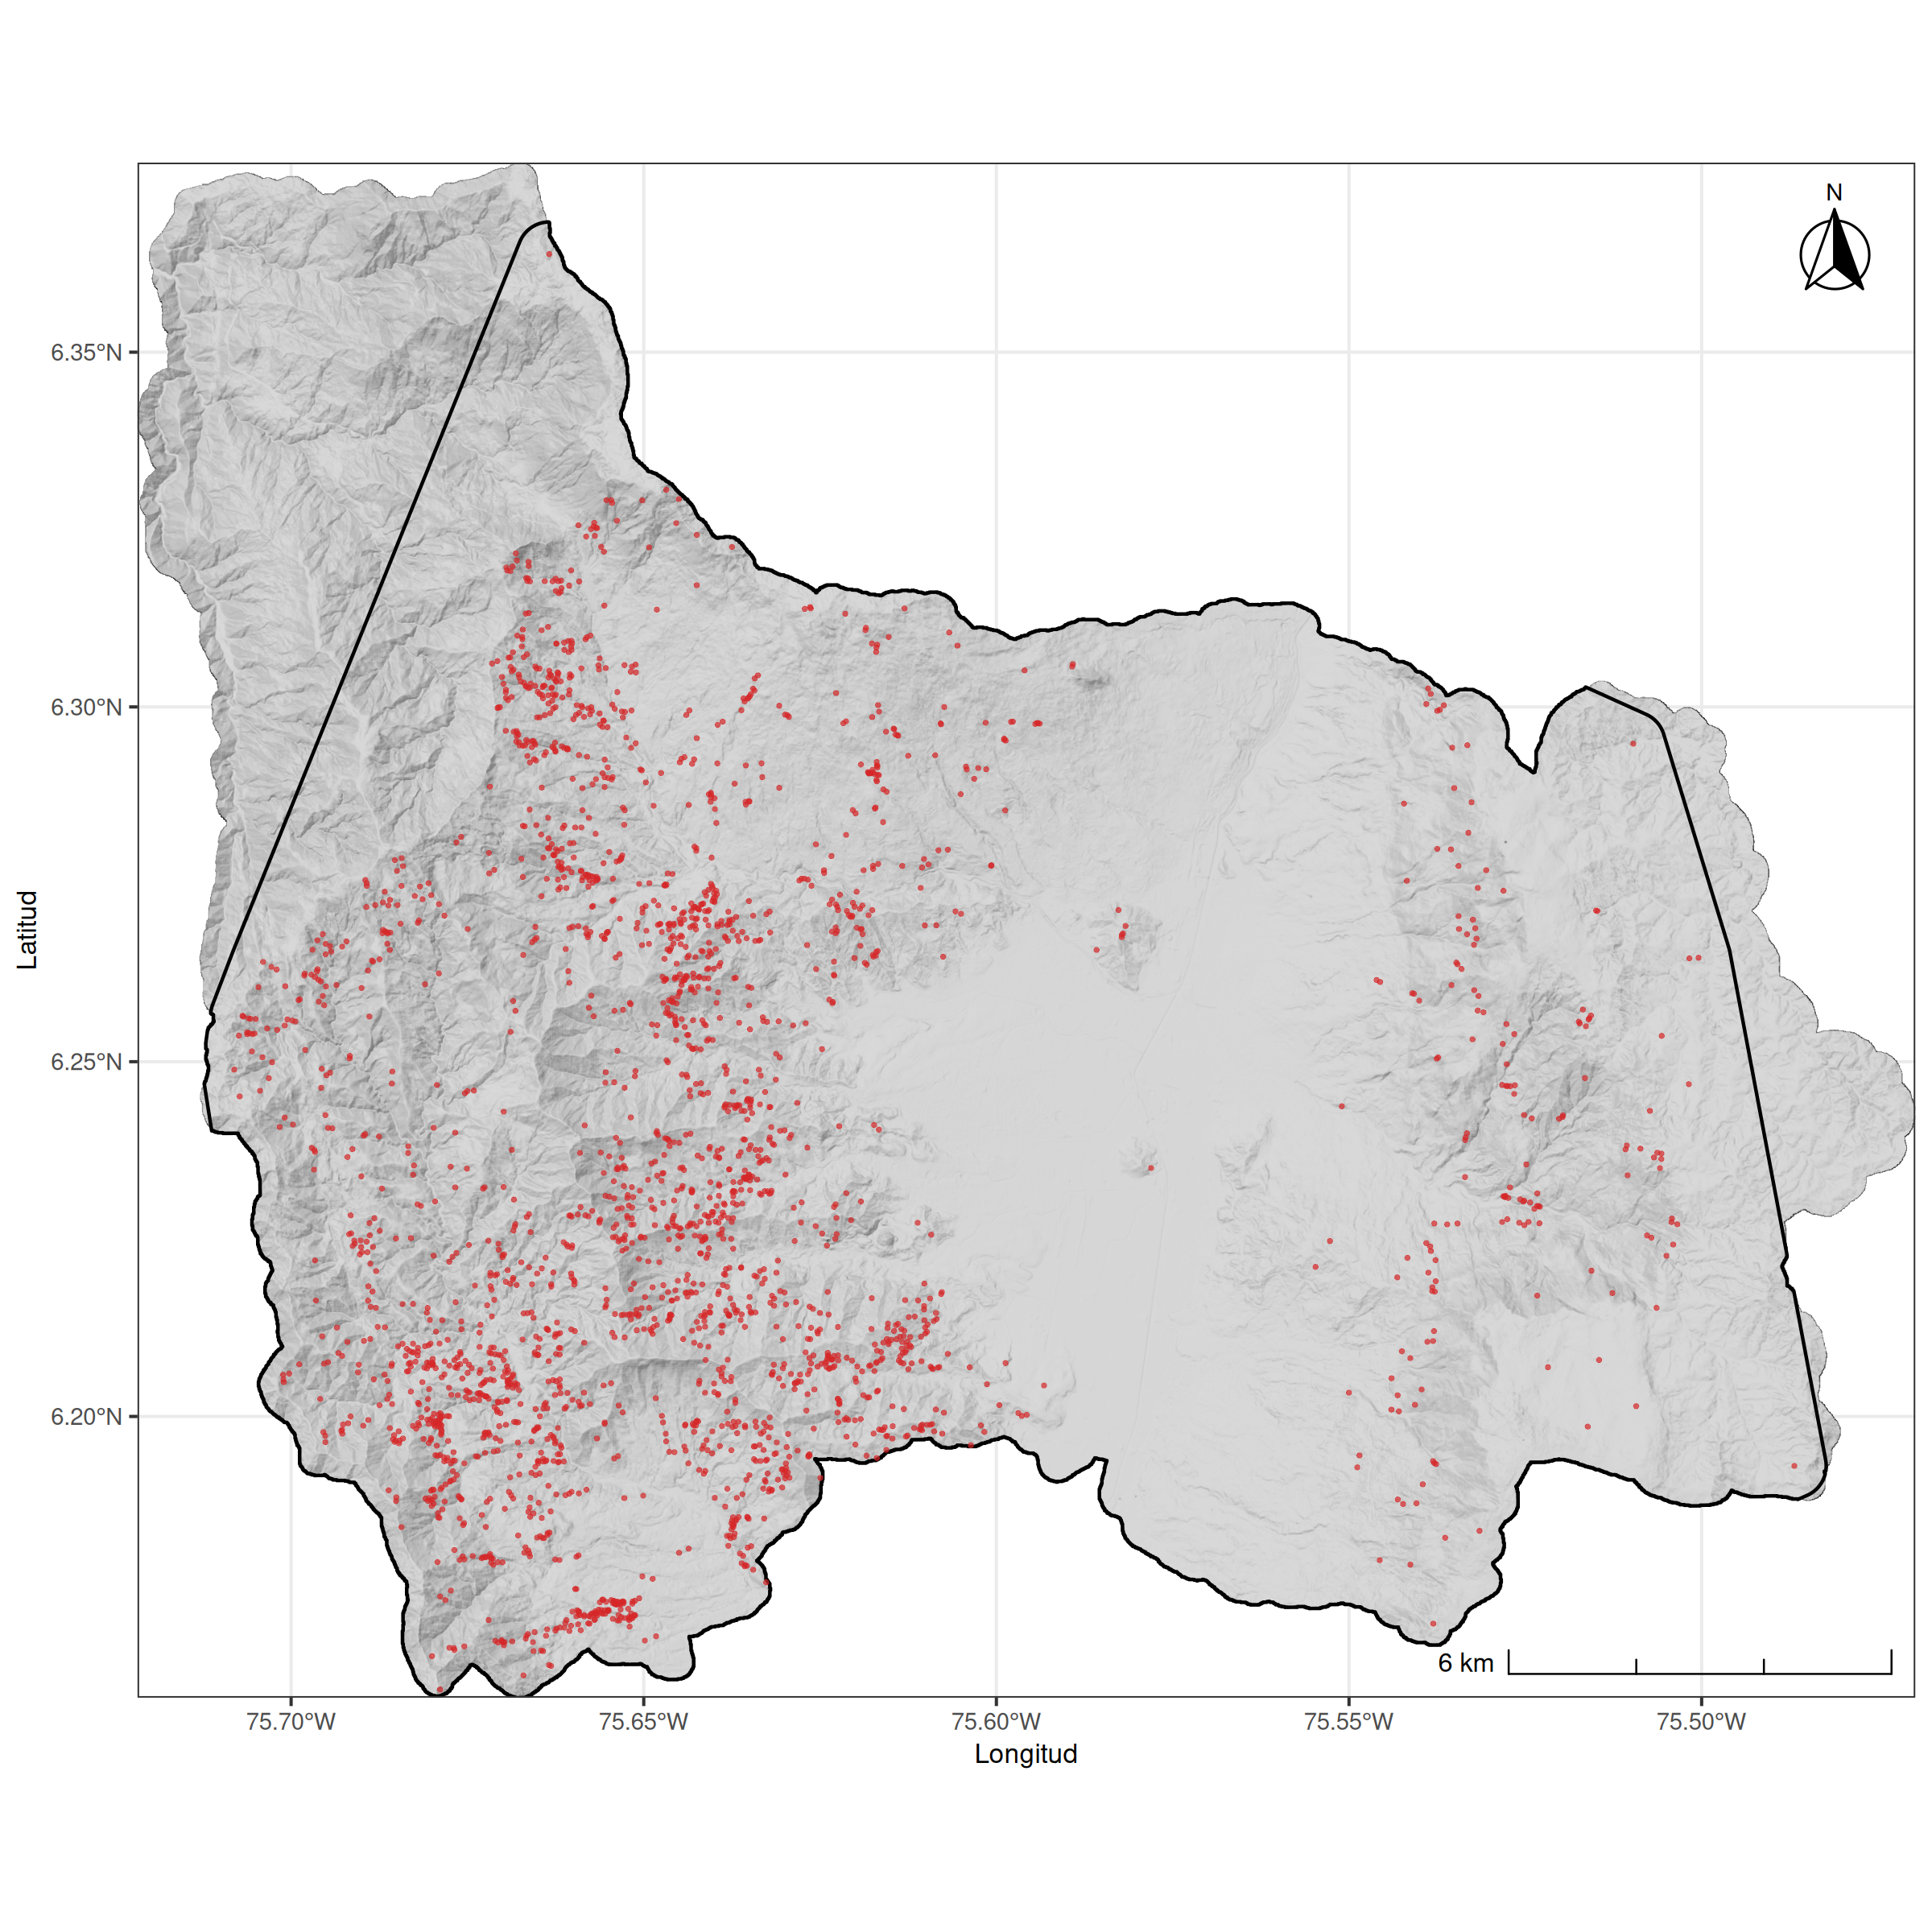
\includegraphics[width=0.95\linewidth]{FIG/00_inventario_deslizamientos.png}
  \caption{Localización espacial de los \num{2504} movimientos en masa
           registrados en el dominio de estudio del Valle de Aburrá. Cada
           punto rojo representa la zona de iniciación de un evento. El
           contorno negro delimita el dominio de estudio $\Omega$
           (\SI{335,21}{km^2}).}
  \label{fig:inventario}
\end{figure}

Se usaron covariables topográficas derivadas de un Modelo Digital de Elevación
(MDE) de \SI{1}{m} de resolución obtenido con tecnología LiDAR, remuestreado a
\SI{2}{m} mediante promediado por agregación para mejorar la relación
señal-ruido en las covariables morfométricas y reducir el costo computacional
(Tabla~\ref{tab:covstats}). La pendiente ($\beta$, grados) se define como el
ángulo de la máxima pendiente descendente. El aspecto ($\alpha$, grados desde el Norte) es la dirección de
la máxima pendiente descendente y controla la exposición solar, la
evapotranspiración y el contenido de humedad del suelo. Las dos covariables
topográficas se estandarizaron a media cero y desviación estándar unitaria
sobre el dominio completo antes del ajuste del modelo.

\begin{table}[htbp]
  \centering
  \caption{Estadísticas descriptivas de las covariables topográficas
           estandarizadas en las \num{2504} localizaciones de movimientos en
           masa (MDE a \SI{2}{m}).}
  \label{tab:covstats}
  \resizebox{\linewidth}{!}{%
  \begin{tabular}{lrrrrr}
    \toprule
    Covariable & Mín. & Q$_{25}$ & Mediana & Q$_{75}$ & Máx. \\
    \midrule
    Pendiente (°) & $0{,}12$ & $28{,}37$ & $36{,}84$ & $43{,}24$ & $65{,}13$ \\
    Aspecto (°)   & $0{,}16$ & $86{,}45$ & $144{,}35$ & $203{,}99$ & $359{,}68$ \\
    \bottomrule
  \end{tabular}}
\end{table}

Por ser un territorio fuertemente antropizado se usaron dos tipos de uso del
suelo: urbano y rural. La incorporación de la geología se realizó categorizando
cada unidad geológica en dos clases binarias: (i) \textit{suelos finos}: incluye esquistos, dunitas, rocas volcánicas y
  depósitos de flujos de lodos. Esta categoría cubre aproximadamente el
  \SI{35}{\percent} del dominio; (ii) \textit{suelos gruesos}: incluye gneis, anfibolitas, granodioritas,
  gabros, migmatitas y depósitos aluviales. Esta categoría cubre el
  \SI{65}{\percent} restante del dominio.

% ─────────────────────────────────────────────────────────────
\section{Metodología}
\label{sec:methods}
% ─────────────────────────────────────────────────────────────

\subsection{Proceso de Poisson No Homogéneo (NHPP)}
\label{sec:ipp}

El inventario de movimientos en masa se trata como una realización de un
proceso puntual espacial en el dominio continuo $\Omega \subset \mathbb{R}^2$,
cuya distribución está gobernada por la función de intensidad
$\lambda(\mathbf{s})$. El modelo adoptado es el Proceso de Poisson No
Homogéneo (NHPP), en el que el reto estadístico es estimar
$\lambda(\mathbf{s})$ en todo el dominio a partir de las \num{2504}
localizaciones observadas, teniendo en cuenta que la intensidad varía con la
topografía, el tipo de suelo y la cobertura del territorio. Formalmente, el
NHPP establece que los eventos son condicionalmente independientes dado la
función de intensidad $\lambda(\mathbf{s})$, y el conteo en cualquier área $A$
sigue $N(A) \sim \text{Poisson}\!\left(\int_A \lambda(\mathbf{s})\,d\mathbf{s}\right)$.
Con una intensidad log-lineal en covariables:
\begin{align}
  \{S_i\} \mid \lambda(\cdot) &\sim
    \text{Poisson-NH}\bigl(\lambda(\mathbf{s})\bigr),
  \label{eq:ipp1}\\
  \log\lambda(\mathbf{s}) &= \eta(\mathbf{s}),
  \label{eq:ipp2}\\
  \eta(\mathbf{s}) &= \beta_0 + \beta_1\,\text{pendiente}(\mathbf{s})
    + \beta_2\,\text{aspecto}(\mathbf{s})\nonumber\\
    &\quad + \beta_3\,\text{geo\_finos}(\mathbf{s})
    + \beta_4\,\text{urb}(\mathbf{s}),
  \label{eq:ipp}
\end{align}
donde $\text{pendiente}$ y $\text{aspecto}$ son las covariables topográficas
estandarizadas (media 0, d.e.\ 1); $\text{geo\_finos} \in \{0,1\}$ el
indicador de suelos finos; y $\text{urb} \in \{0,1\}$ el indicador de
cobertura urbanizada.

Los coeficientes $\beta_j$ actúan sobre la \emph{log-intensidad}:
$\beta_j > 0$ implica mayor intensidad esperada al aumentar la covariable $j$.
Un incremento de una desviación estándar en una covariable continua multiplica
la intensidad local por $e^{\beta_j}$. Para covariables binarias, $e^{\beta_j}$
es la razón de intensidades entre la clase activa y la de referencia,
controlando el resto.

La estimación estadística de los coeficientes $\beta_j$ del NHPP requiere
caracterizar la distribución posterior conjunta de todos los parámetros dado el
patrón observado de deslizamientos. La función de verosimilitud del proceso
puntual cuantifica esta compatibilidad: penaliza configuraciones que predicen
alta intensidad donde no ocurrieron eventos, y baja intensidad donde sí los
hay. Su evaluación involucra la integral de la intensidad
$\int_\Omega \lambda(\mathbf{s})\,d\mathbf{s}$ sobre el dominio continuo, que
no tiene solución analítica cuando la intensidad varía en el espacio según
covariables continuas; esta integral se aproxima numéricamente mediante el
dispositivo de Berman-Turner \cite{diggle2013} sobre una malla triangular.

La estimación bayesiana completa de los parámetros requeriría en principio el
muestreo por cadenas de Markov (MCMC), cuyas iteraciones resultan
computacionalmente prohibitivas al evaluar la integral sobre una malla de
\num{92657} nodos. Por ello, se adopta la \emph{Aproximación de Laplace
Anidada Integrada} (INLA) \cite{rue2009, rue2017}, que computa las
distribuciones marginales posteriores de todos los parámetros mediante
aproximaciones analíticas de Laplace, sin simulación estocástica, con precisión
comparable al MCMC y sin el costo computacional.

La malla triangular cubre tanto el dominio interior como un buffer exterior de
\SI{2}{km} (Fig.~\ref{fig:mesh}, Tabla~\ref{tab:mesh}). La malla es necesaria
para aproximar numéricamente la integral
$\int_\Omega \lambda(\mathbf{s})\,d\mathbf{s}$ de la ec.~\eqref{eq:ipp1}
mediante el dispositivo de Berman-Turner \cite{diggle2013}: los nodos de la
malla actúan como puntos de integración con pesos proporcionales al área de la
celda de Voronoi dual. Las aristas interiores de hasta \SI{100}{m} proporcionan
suficiente resolución para representar la variabilidad espacial de las
covariables a \SI{2}{m}. El buffer exterior reduce los artefactos de borde.

\begin{table}[htbp]
  \centering
  \caption{Parámetros de la malla triangular utilizada para la integración
           numérica de la verosimilitud del NHPP
           (dispositivo de Berman-Turner).}
  \label{tab:mesh}
  \begin{tabular}{lrr}
    \toprule
    Parámetro & Valor & Unidad \\
    \midrule
    Arista máxima (interior)      & 100     & m \\
    Arista máxima (exterior)      & 500     & m \\
    Separación mínima entre nodos & 20      & m \\
    Offset interior               & 200     & m \\
    Offset exterior               & 2\,000  & m \\
    Número de nodos               & 92\,657  & -- \\
    Número de triángulos          & 185\,024 & -- \\
    \bottomrule
  \end{tabular}
\end{table}

El modelo se implementó en el lenguaje R \cite{rcore2024}, utilizando los
paquetes \texttt{INLA} \cite{rue2017}, \texttt{inlabru} \cite{bachl2019},
\texttt{fmesher}, \texttt{sf} y \texttt{terra}. Los coeficientes de regresión
recibieron priors débilmente informativos: $\beta_j \sim \mathcal{N}(0,1)$,
lo que implica que un incremento unitario en una covariable se asocia a priori
con un factor de intensidad de $e^{\pm 1} \approx 2{,}7$ en cualquier
dirección. Los mapas predictivos de $\lambda(\mathbf{s})$ se obtuvieron sobre
grillas de \SI{100}{m} con \num{500} muestras de Monte Carlo de la posterior
conjunta. El desempeño discriminativo se evaluó con el AUC calculado sobre una
grilla hexagonal de $\approx$\,\SI{0,25}{km^2}, asignando a cada celda un
indicador binario (1 si contenía al menos un evento) y como puntuación la
intensidad total predicha.

% ─────────────────────────────────────────────────────────────
\section{Resultados}
\label{sec:results}
% ─────────────────────────────────────────────────────────────

La distribución de movimientos en masa de acuerdo con el inventario es
marcadamente no homogénea, con densidades locales que superan los
20~eventos~km$^{-2}$ en los flancos de mayor pendiente del valle. La
Fig.~\ref{fig:inventario} muestra la distribución espacial de los eventos y la
Fig.~\ref{fig:mesh} la malla triangular de integración.

De los \num{2504} eventos, la densidad de eventos por km$^2$ es
notablemente mayor en suelos finos. La distribución espacial del inventario
refleja fundamentalmente los patrones topográficos del Valle de Aburrá, sin la
concentración en zonas urbanas que caracteriza a los inventarios históricos;
esto es indicativo de que el inventario de sensores remotos captura
efectivamente la variabilidad espacial de la susceptibilidad a escala de
ladera.

\begin{figure}[htbp]
  \centering
  \includegraphics[width=0.95\linewidth]{FIG/2m_01_mesh.png}
  \caption{Malla triangular superpuesta al hillshade del relieve de Medellín.
           Puntos rojos: zonas de iniciación de movimientos en masa observados
           (\num{2504} eventos). Triangulación azul: malla de integración
           (\num{92657} nodos, \num{185024} triángulos). El buffer exterior
           (triángulos de mayor tamaño) se extiende \SI{2}{km} fuera del
           dominio de estudio (contorno negro) para atenuar los efectos de
           borde en la integración numérica.}
  \label{fig:mesh}
\end{figure}

La Tabla~\ref{tab:fixeff} y la Fig.~\ref{fig:fixeff} presentan los coeficientes
posteriores del modelo NHPP. La pendiente es el único predictor topográfico
positivo y significativo; el aspecto muestra un efecto negativo significativo.
Los dos predictores binarios (suelos finos y cobertura urbana) son negativos y
significativos.

\begin{table}[htbp]
  \centering
  \caption{Resumen posterior de los efectos fijos del modelo NHPP (MDE a
           \SI{2}{m}, covariables estandarizadas). Los coeficientes indican el
           cambio en $\log\lambda(\mathbf{s})$ por incremento de una
           desviación estándar en cada covariable continua, o el efecto de
           pertenecer a la clase activa para las variables binarias.}
  \label{tab:fixeff}
  \resizebox{\linewidth}{!}{%
  \begin{tabular}{lrrrr}
    \toprule
    Predictor & Media & D.E. & IC$_{2{,}5\%}$ & IC$_{97{,}5\%}$ \\
    \midrule
    Intercepto          & $-11{,}769$ & $0{,}034$ & $-11{,}835$ & $-11{,}703$ \\
    Pendiente (estand.) & $\phantom{-}0{,}901$ & $0{,}023$
                        & $\phantom{-}0{,}856$ & $\phantom{-}0{,}946$ \\
    Aspecto (estand.)   & $-0{,}243$  & $0{,}020$ & $-0{,}283$  & $-0{,}204$ \\
    Cob.\ urbana        & $-0{,}971$  & $0{,}093$ & $-1{,}154$  & $-0{,}788$ \\
    Suelos finos (bin.) & $-0{,}709$  & $0{,}041$ & $-0{,}790$  & $-0{,}628$ \\
    \bottomrule
  \end{tabular}}
\end{table}

\begin{figure}[htbp]
  \centering
  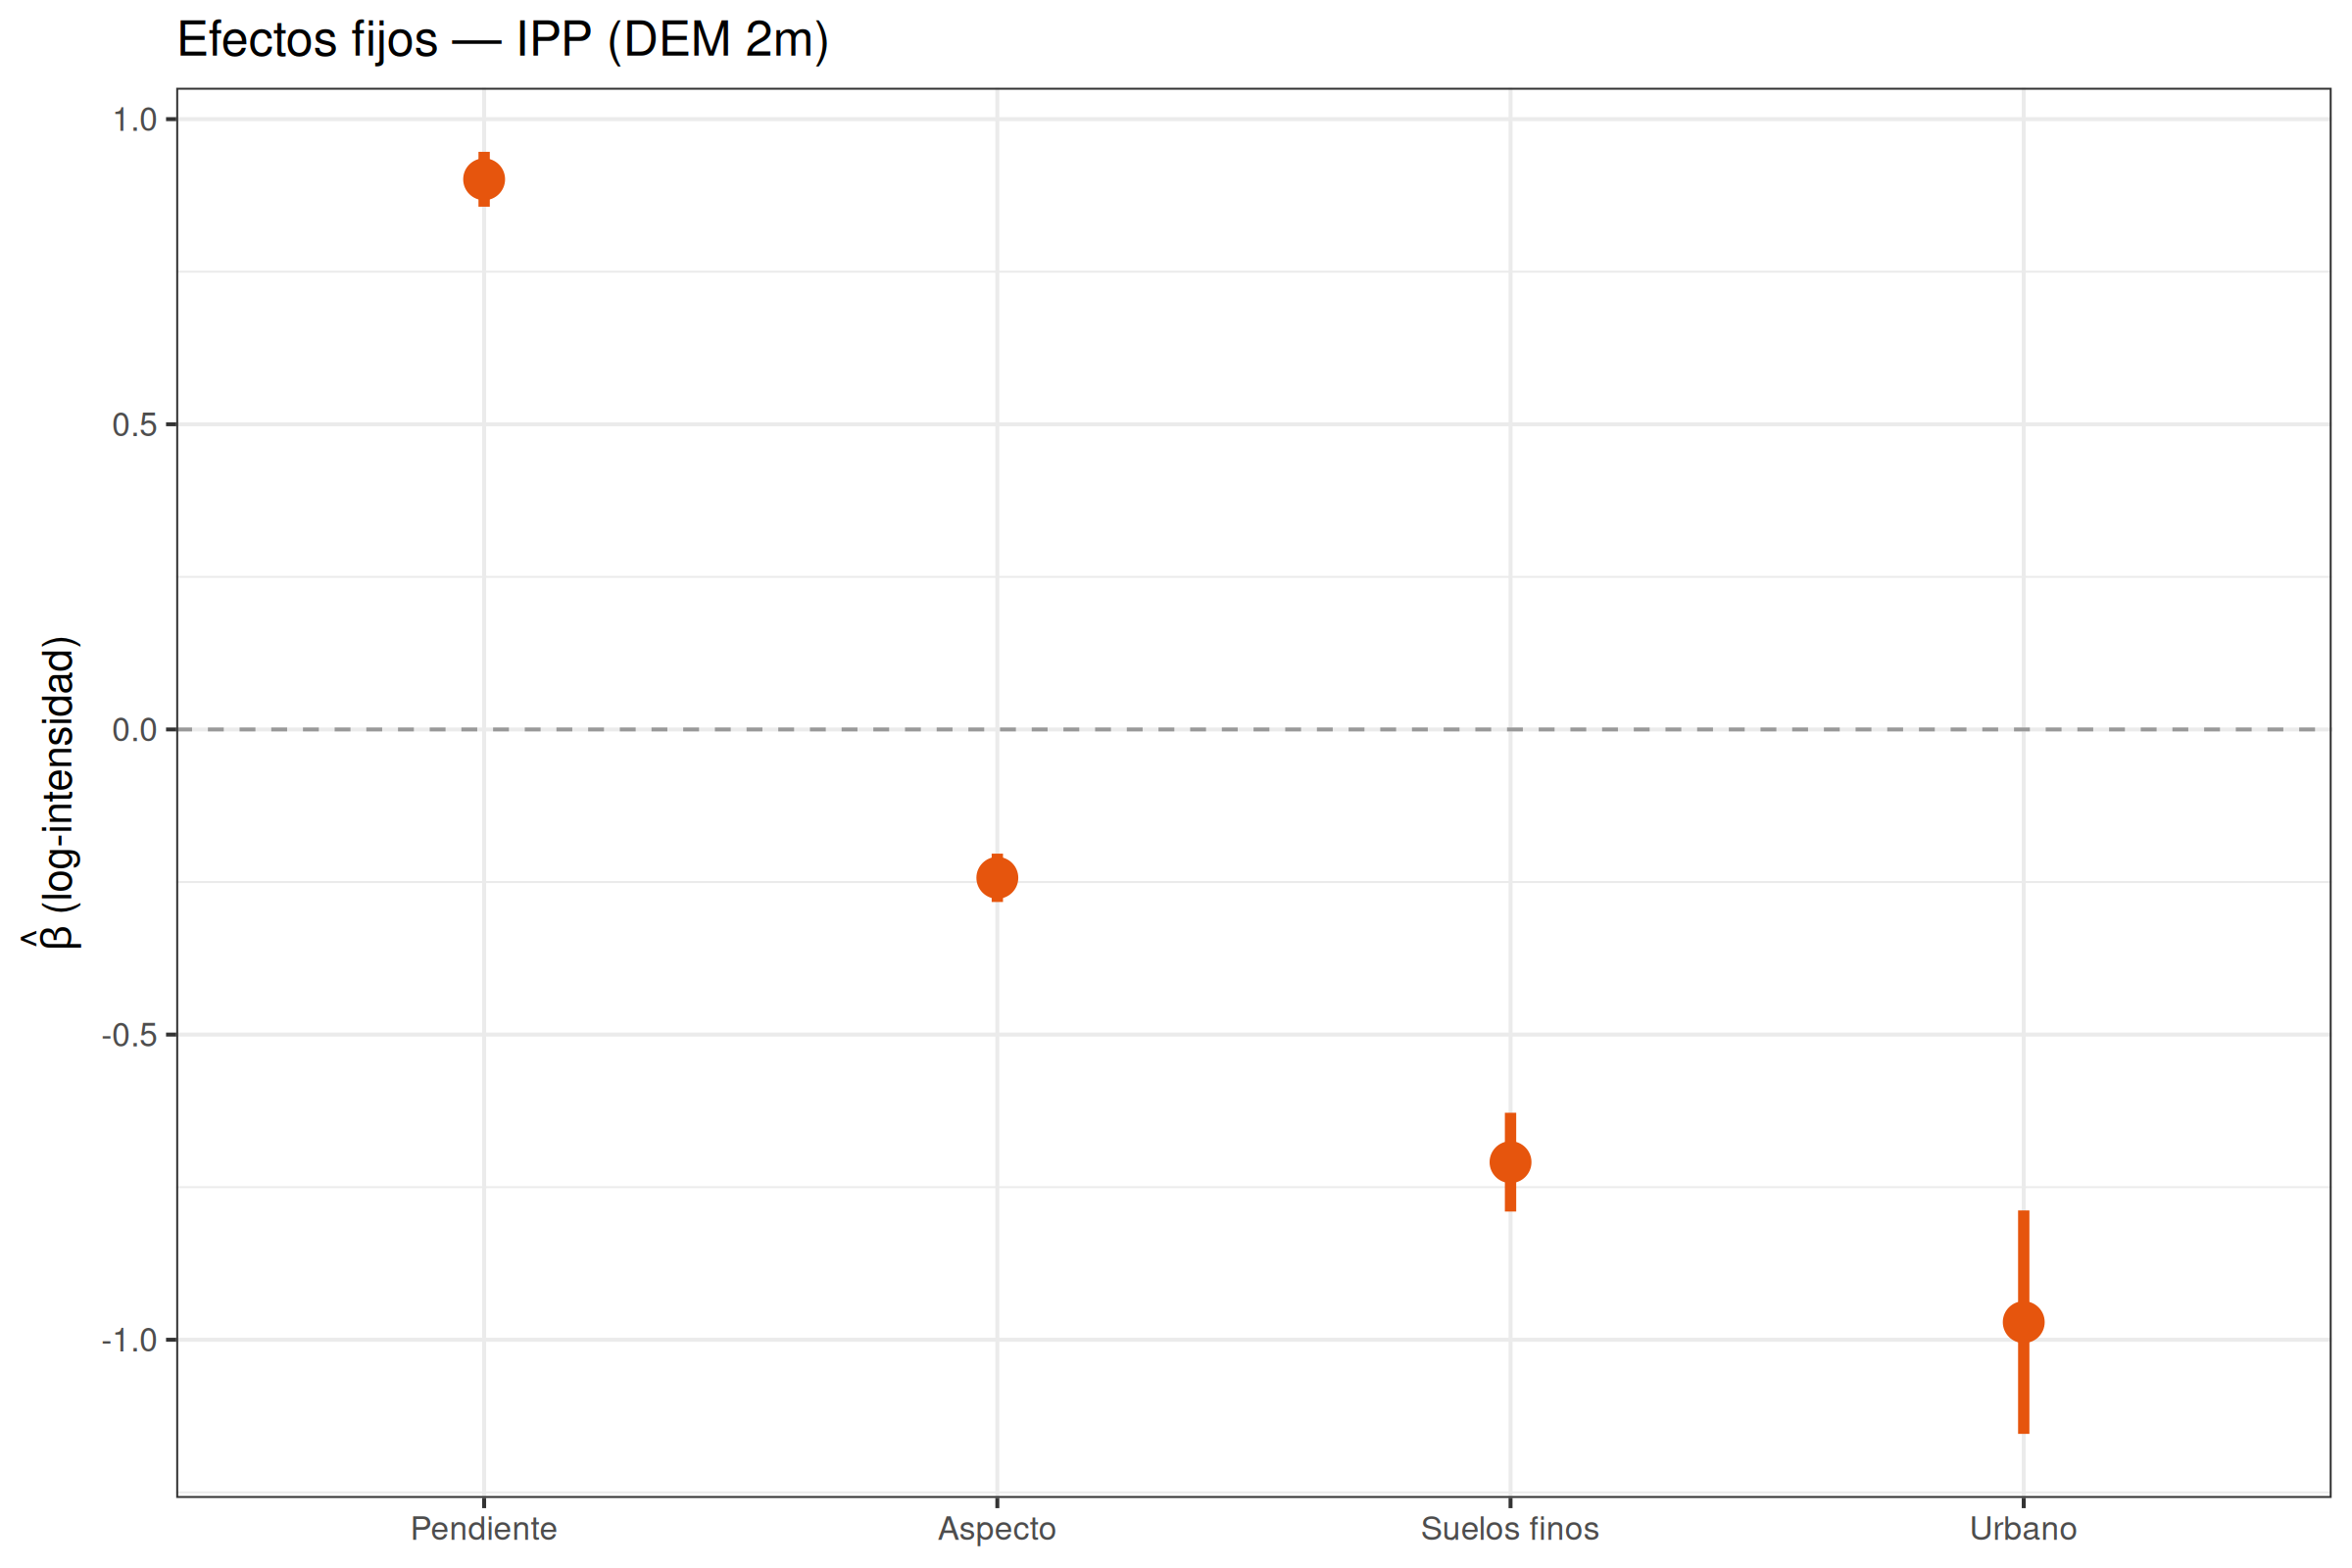
\includegraphics[width=0.95\linewidth]{FIG/2m_02_efectos_fijos.png}
  \caption{Medias posteriores e intervalos de credibilidad al 95\,\% de los
           coeficientes de efectos fijos $\hat{\beta}$ (escala log-intensidad)
           del modelo NHPP (MDE \SI{2}{m}). La pendiente es el predictor
           positivo dominante; aspecto, cobertura urbana y suelos finos
           muestran efectos negativos significativos.}
  \label{fig:fixeff}
\end{figure}

\textbf{Pendiente} ($\hat{\beta}_1 = 0{,}901$;
IC$_{95\%}$: $[0{,}856;\,0{,}946]$): el coeficiente es positivo,
coherente con el papel mecánico fundamental de la pendiente.

\textbf{Aspecto} ($\hat{\beta}_2 = -0{,}243$;
IC$_{95\%}$: $[-0{,}283;\,-0{,}204]$): el coeficiente negativo indica mayor
susceptibilidad en laderas de orientación norte.

\textbf{Suelos finos} ($\hat{\beta}_3 = -0{,}709$;
IC$_{95\%}$: $[-0{,}790;\,-0{,}628]$): coeficiente negativo al parecer
controlado por la topografía. Este resultado sugiere que la mayor
susceptibilidad de los suelos finos está mediada casi completamente por su
topografía asociada (pendientes más elevadas en el estrato fino), y que una
vez que se controlan esas covariables el efecto litológico directo es débil o
de signo contrario al esperado.

\textbf{Cobertura urbana} ($\hat{\beta}_4 = -0{,}971$;
IC$_{95\%}$: $[-1{,}154;\,-0{,}788]$): el coeficiente es significativamente
negativo. Los sectores clasificados como urbanos muestran una intensidad
predicha significativamente menor que las zonas rurales una vez que se controla
la topografía. Este resultado refleja que las zonas urbanas de Medellín se
localizan predominantemente en el fondo plano del valle (baja pendiente) y que
el indicador binario captura el efecto residual de la urbanización, que en
pendientes bajas reduce la susceptibilidad respecto a laderas rurales.

La Fig.~\ref{fig:maps} muestra la superficie de intensidad media posterior
$\hat{\lambda}(\mathbf{s})$ y su incertidumbre en el dominio de estudio. Las
áreas de mayor intensidad (colores rojos) se localizan a lo largo de los
flancos del río Medellín y sus tributarios principales, donde la combinación de
alta pendiente y orientación norte maximiza el predictor lineal. Los colores
verdes indican baja susceptibilidad, correspondientes al fondo plano del valle
y a las zonas urbanas. La distribución espacial de la incertidumbre posterior
refleja el número local de eventos: zonas con alta densidad de deslizamientos
exhiben menor varianza predictiva.

\begin{figure*}[!t]
  \centering
  \begin{subfigure}[b]{0.48\linewidth}
    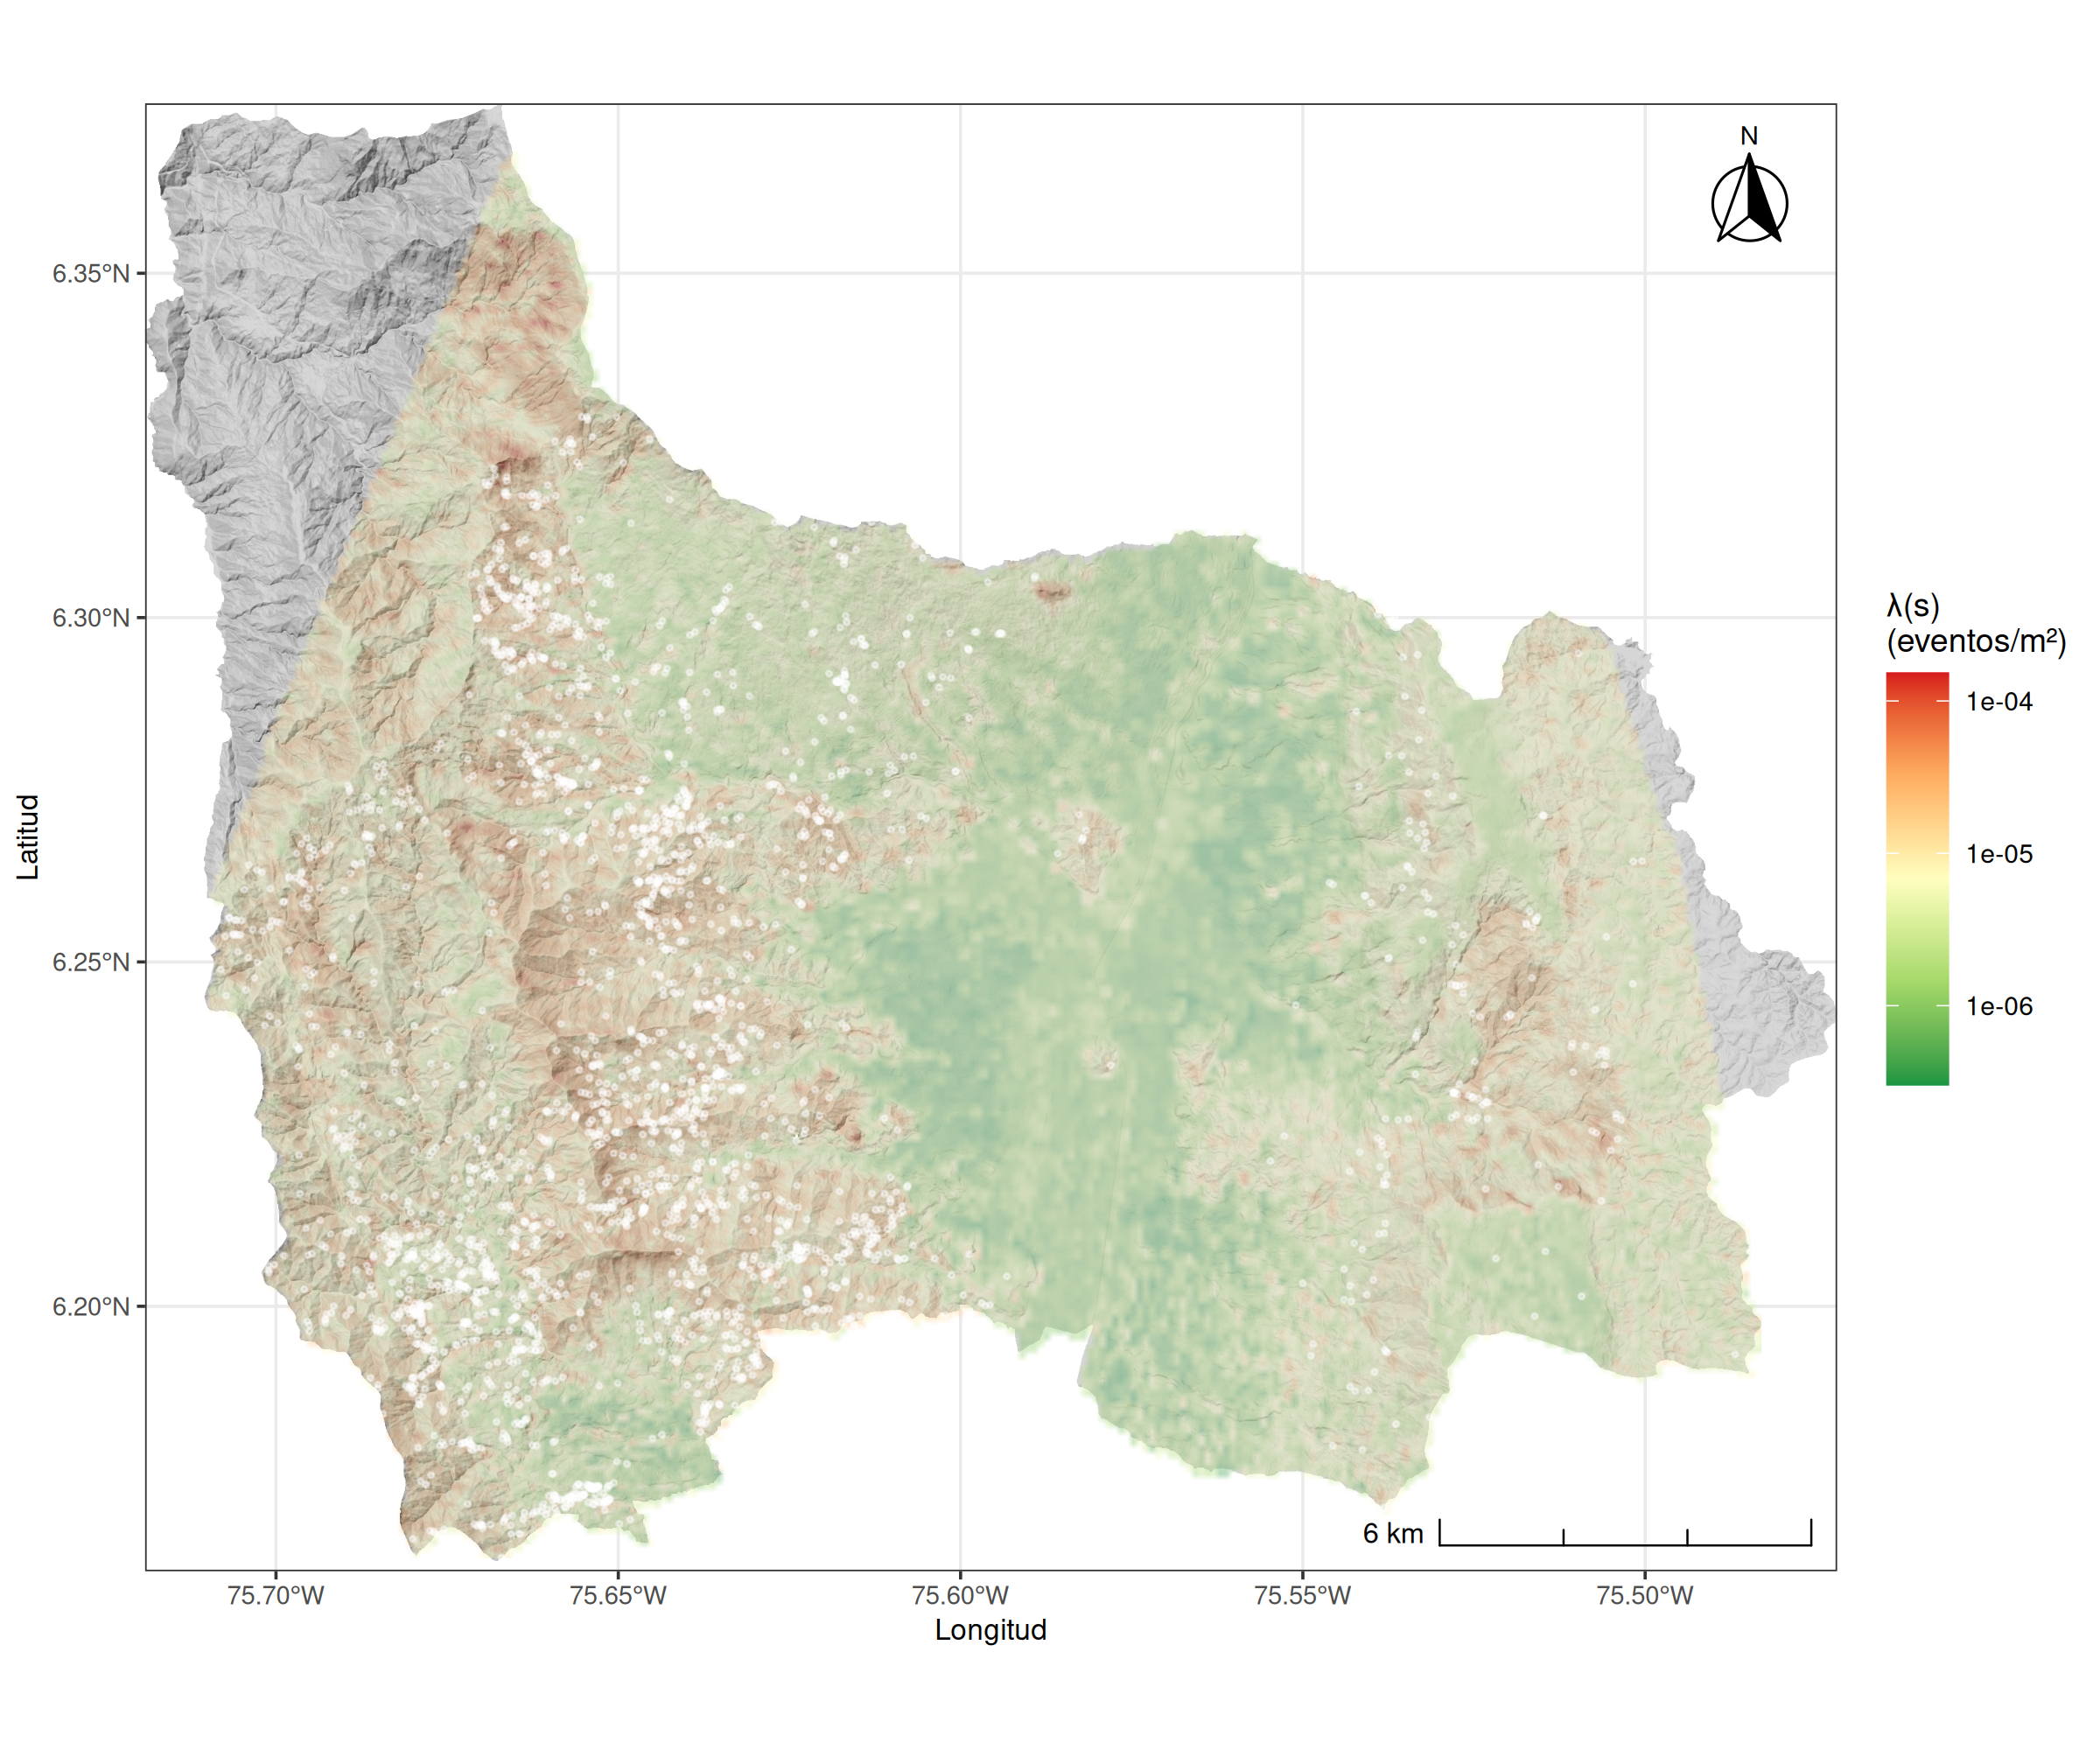
\includegraphics[width=\linewidth]{FIG/2m_04_intensidad.png}
    \caption{Intensidad media posterior $\hat{\lambda}(\mathbf{s})$.}
    \label{fig:intensity}
  \end{subfigure}
  \hfill
  \begin{subfigure}[b]{0.48\linewidth}
    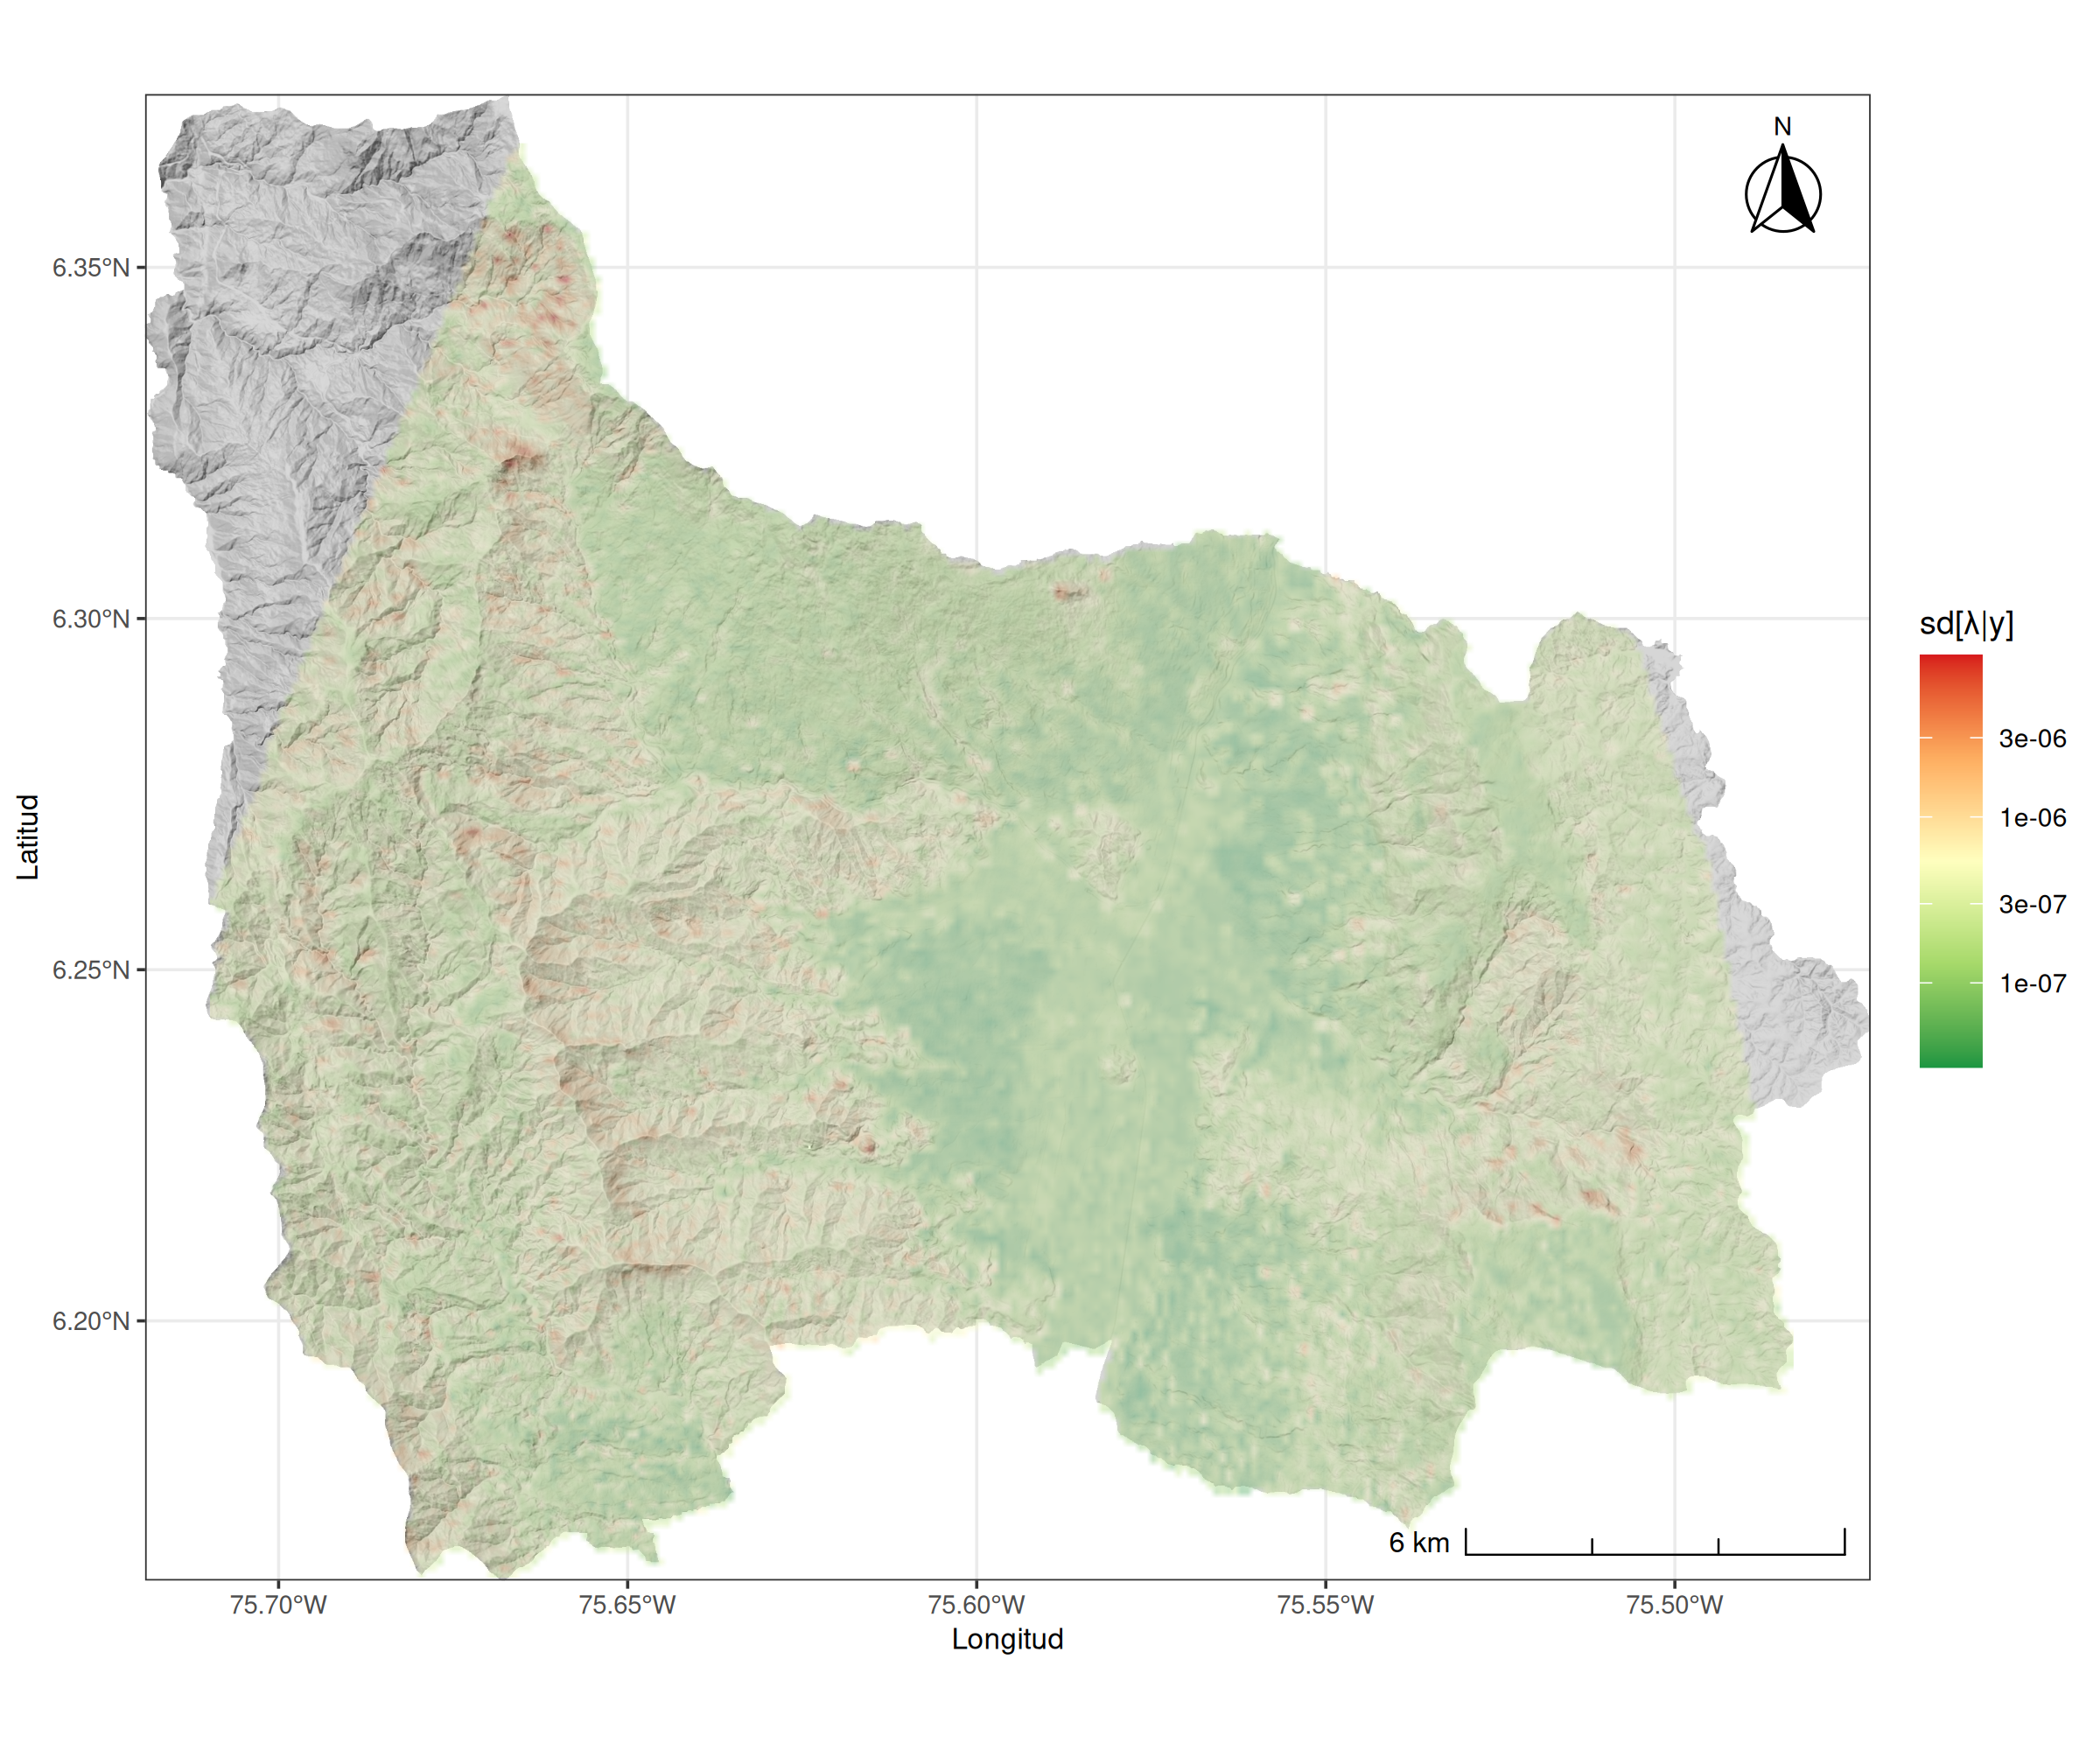
\includegraphics[width=\linewidth]{FIG/2m_05_incertidumbre.png}
    \caption{Desviación estándar posterior.}
    \label{fig:uncertainty}
  \end{subfigure}
  \caption{Mapas de (a) la intensidad media posterior $\hat{\lambda}(\mathbf{s})$
           (eventos~m$^{-2}$) y (b) la desviación estándar posterior del modelo
           NHPP en el Valle de Aburrá. (a) Verde: baja susceptibilidad; rojo:
           alta susceptibilidad (escala logarítmica). (b) De violeta a amarillo:
           baja a alta incertidumbre en la estimación de $\lambda(\mathbf{s})$.}
  \label{fig:maps}
\end{figure*}

El mapa de residuos de Pearson
$(n_{\text{obs}} - n_{\text{esp}})/\sqrt{n_{\text{esp}}}$
(Fig.~\ref{fig:residuos}) no muestra un patrón espacial sistemático con
estructura geográfica definida, lo que indica que el modelo no presenta sesgo
espacial evidente. Los residuos positivos más pronunciados se concentran
puntualmente en algunas quebradas, posiblemente donde los registros históricos
son incompletos o donde factores antrópicos locales amplifican la
susceptibilidad.

\begin{figure}[htbp]
  \centering
  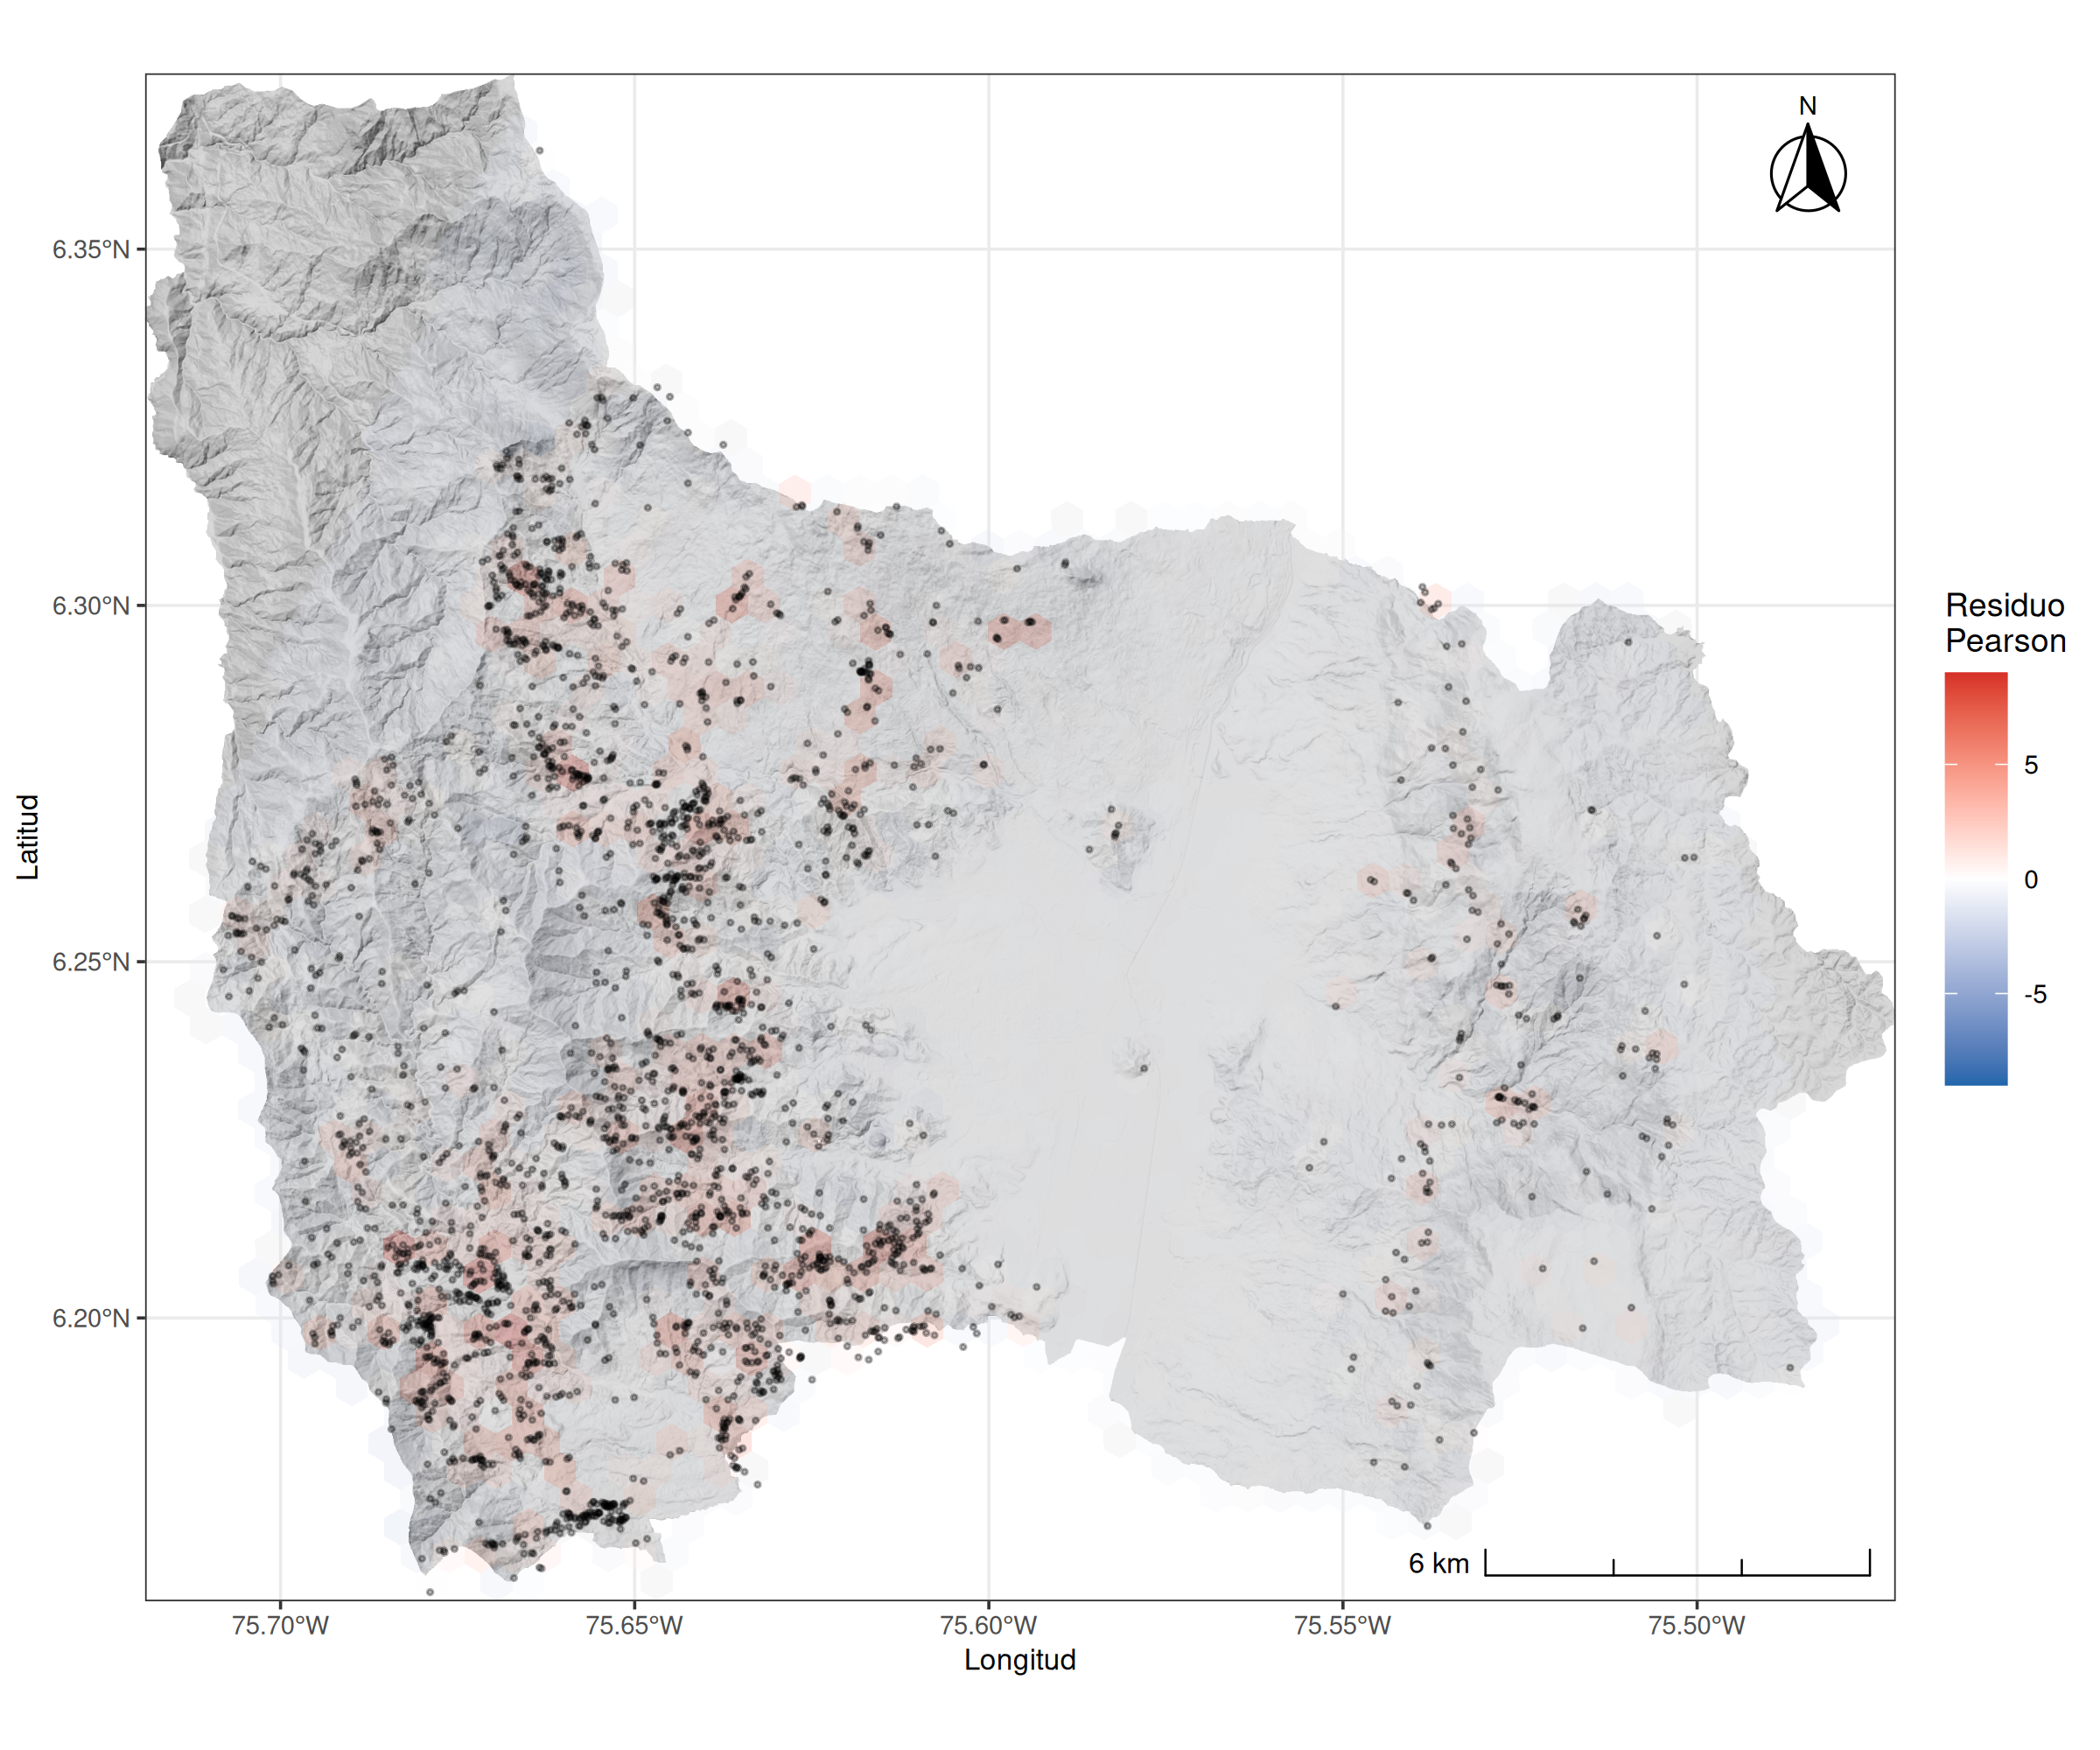
\includegraphics[width=0.95\linewidth]{FIG/2m_09_residuos.png}
  \caption{Mapa de residuos de Pearson
           $(n_{\text{obs}} - n_{\text{esp}})/\sqrt{n_{\text{esp}}}$ del
           modelo NHPP sobre el Valle de Aburrá. Rojo: celdas con más eventos
           de los esperados (posible subestimación de la susceptibilidad local
           o subreporte en el inventario). Azul: celdas con menos eventos de
           los esperados.}
  \label{fig:residuos}
\end{figure}

La Tabla~\ref{tab:diagnostics} resume las métricas de ajuste del modelo. El
modelo clasifica correctamente una
celda con movimiento en masa por encima de una celda sin evento en
aproximadamente el 76\,\% de los casos. La Fig.~\ref{fig:roc} muestra la curva
ROC completa.

\begin{table}[htbp]
  \centering
  \caption{Métricas de ajuste del modelo NHPP sobre el dominio completo
           (MDE \SI{2}{m}, cuatro predictores).}
  \label{tab:diagnostics}
  \begin{tabular}{lr}
    \toprule
    Métrica & Valor \\
    \midrule
    AUC (ROC)               & $0{,}762$ \\
    Número total de eventos & $2\,504$ \\
    Intensidad media        & $7{,}08$ eventos km$^{-2}$ \\
    Área del dominio        & \SI{335,21}{km^2} \\
    \bottomrule
  \end{tabular}
\end{table}

\begin{figure}[htbp]
  \centering
  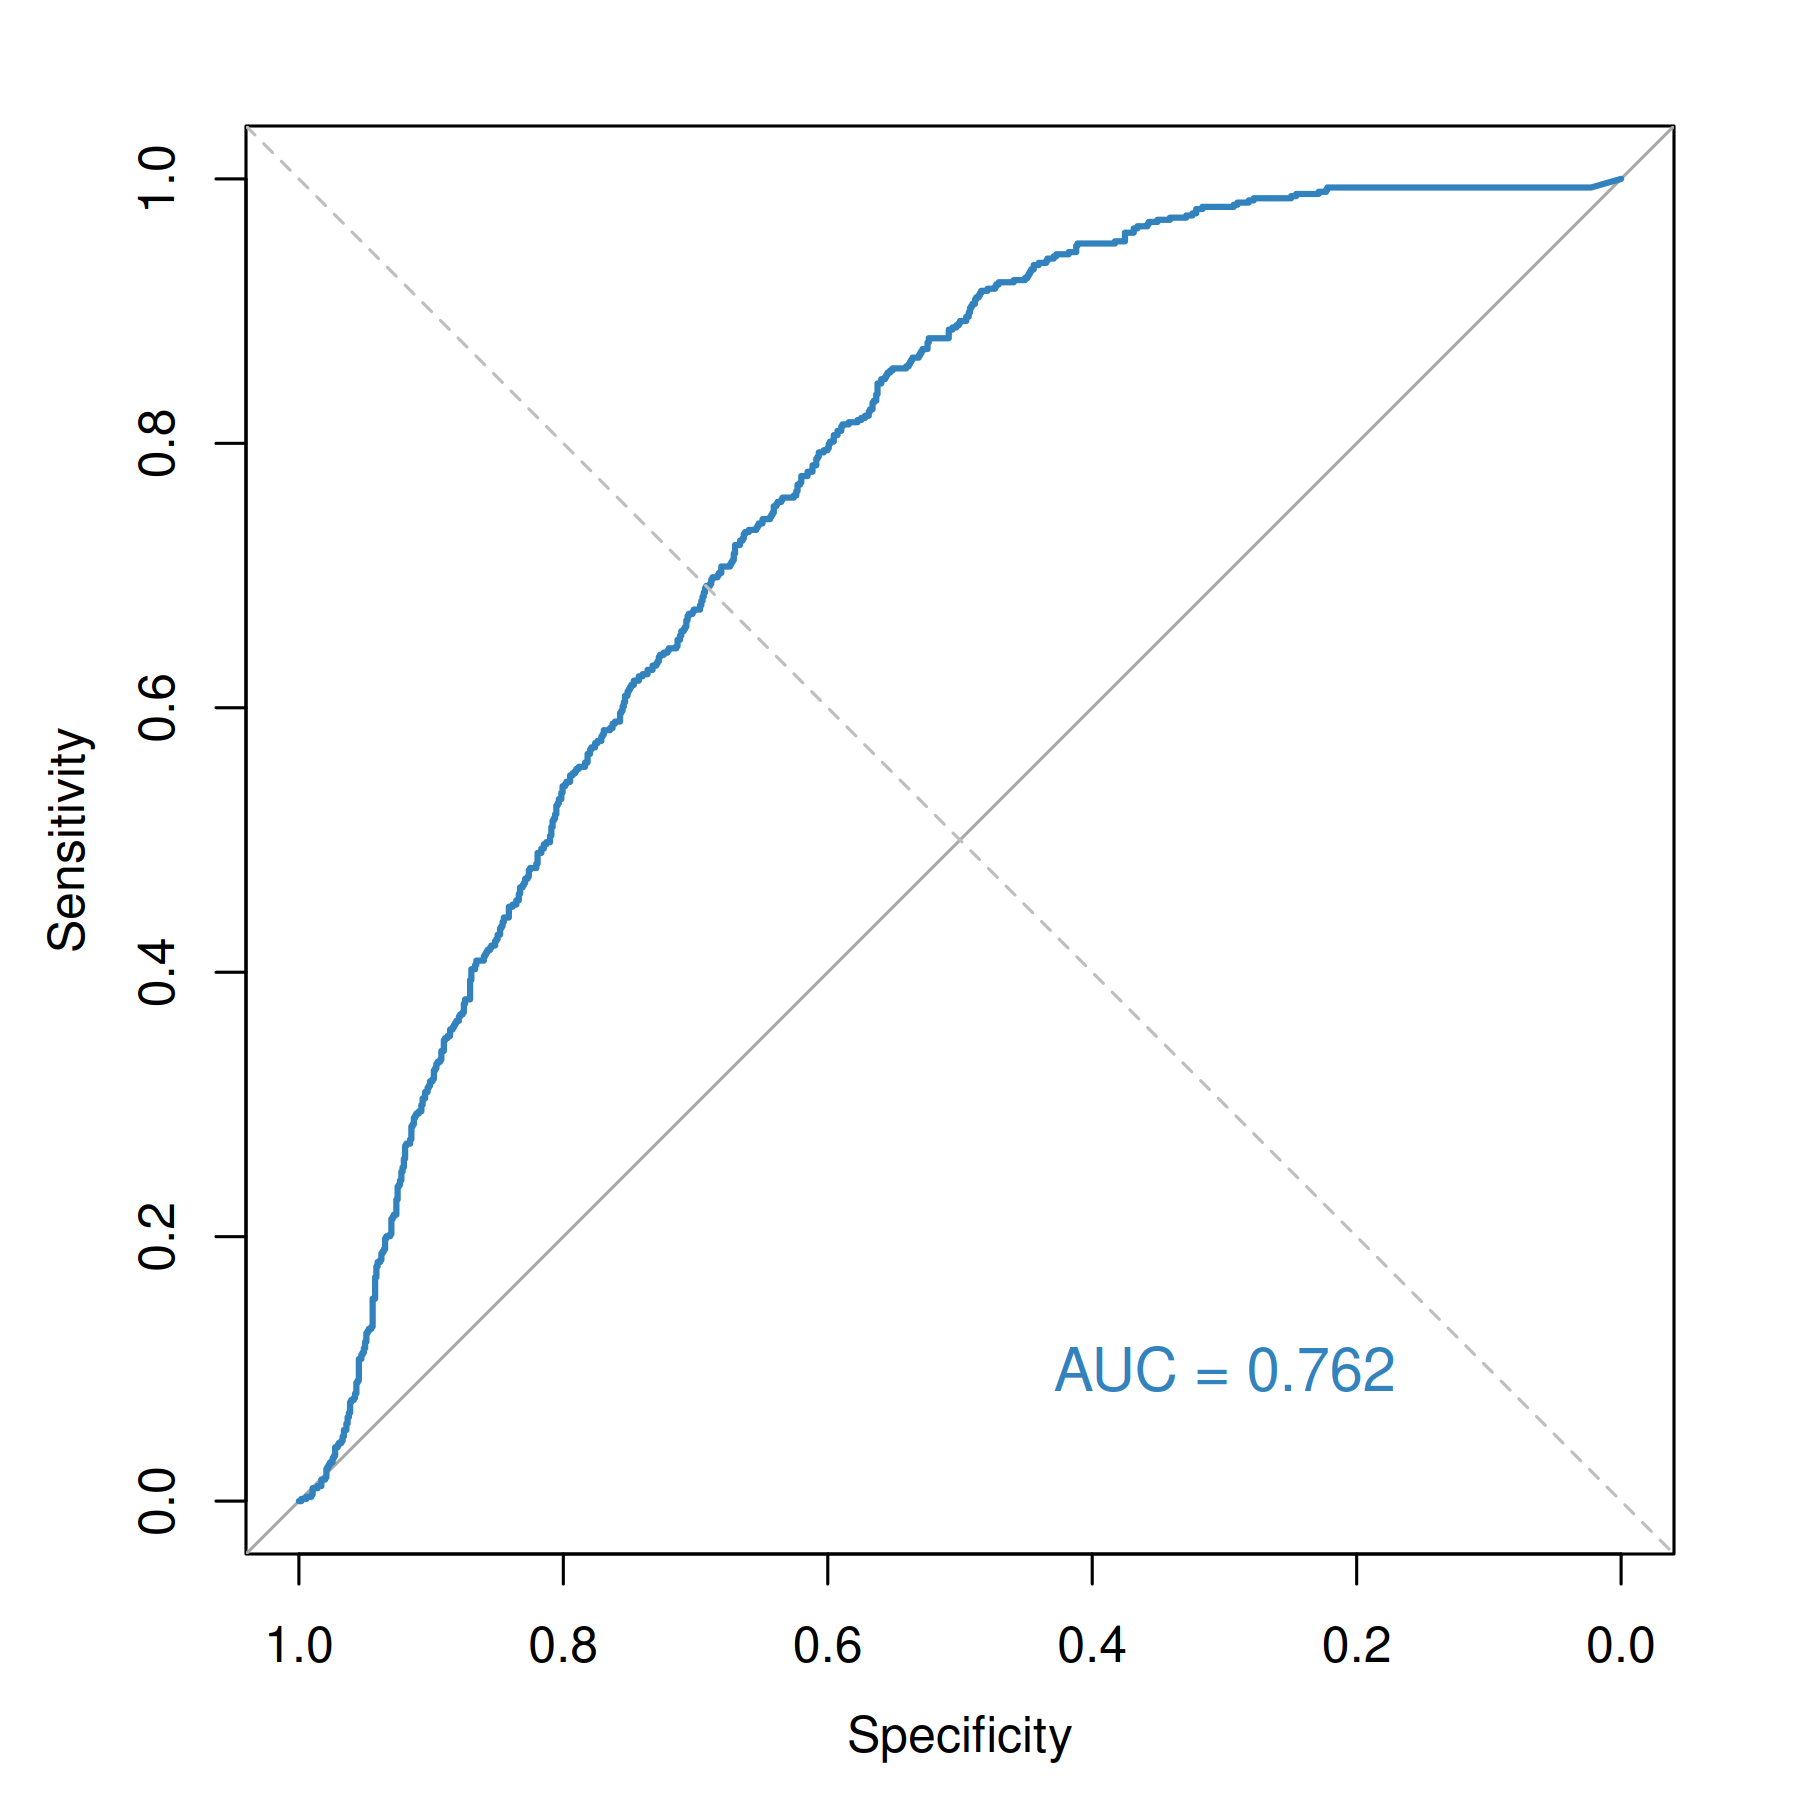
\includegraphics[width=0.85\linewidth]{FIG/2m_12_roc.png}
  \caption{Curva ROC del modelo NHPP evaluada sobre una grilla hexagonal de
           $\approx 0{,}25\,\text{km}^2$ en el dominio completo. El eje
           horizontal es la tasa de falsos positivos y el vertical la tasa de
           verdaderos positivos. La línea diagonal punteada representa un
           clasificador aleatorio (AUC~$=0{,}5$).}
  \label{fig:roc}
\end{figure}

% ─────────────────────────────────────────────────────────────
\section{Discusión}
\label{sec:discussion}
% ─────────────────────────────────────────────────────────────

La susceptibilidad a los movimientos en masa puede modelarse mediante
distribuciones de Poisson bajo dos paradigmas espaciales que conviene
contrastar. El \emph{modelo de área} agrega los eventos en polígonos discretos
y modela el conteo $y_i$
en la unidad $i$ como $y_i \sim \text{Poisson}(\lambda_i A_i)$
\cite{aristizabal2025ag}. Sus ventajas son la eficiencia
computacional y la interpretabilidad directa de los efectos aleatorios espaciales como variaciones
regionales de la susceptibilidad no explicadas por los predictores fijos. La
principal limitación es que la intensidad estimada es constante dentro de cada
polígono independientemente de la variabilidad topográfica interna, y que los
resultados dependen del tamaño y la forma de las unidades de análisis elegidas,
lo que puede introducir discontinuidades artificiales en los límites de los
polígonos.

El proceso puntual espacial adoptado en este trabajo supera estas limitaciones
estructurales. La función de intensidad $\lambda(\mathbf{s})$ varía de forma
continua en cada coordenada del dominio, utilizando las covariables exactas en
ese punto y produciendo una superficie de susceptibilidad suave sin
discontinuidades en los límites de polígonos ni dependencia del tamaño de las
unidades de análisis. En los Andes, donde la pendiente puede cambiar en
distancias de pocos metros, esta propiedad es fundamental para representar
fielmente la distribución espacial de la amenaza a escala de ladera. Además, el
NHPP no requiere \emph{offset} de área ---la integral
$\int_A \lambda(\mathbf{s})\,d\mathbf{s}$ da directamente el número esperado
de eventos en cualquier región $A$--- ni demanda definir celdas sin
deslizamientos. La contrapartida es un mayor costo computacional: la integral
$\int_\Omega \lambda(\mathbf{s})\,d\mathbf{s}$ se evalúa numéricamente sobre
una malla triangular (\num{92657} nodos en este trabajo) y la inferencia
requiere la aproximación bayesiana INLA para ser factible en tiempos razonables.
La elección entre ambos paradigmas depende de la escala de análisis y los
objetivos del estudio: el modelo de área es adecuado a escalas regionales con
unidades geográficas relativamente homogéneas, mientras que el proceso puntual
es preferible cuando se dispone de inventarios de alta resolución y se requiere
estimar la susceptibilidad con resolución métrica en terrenos topográficamente
complejos.

En cuanto a los resultados, los coeficientes del modelo confirman que la
topografía es el principal determinante de la distribución espacial de los
movimientos en masa en Medellín. El coeficiente de pendiente
$\hat{\beta}_1 = 0{,}901$ es positivo y de gran magnitud, reflejando que las
fuertes pendientes son el determinante primario de la
inestabilidad. Un incremento de una desviación estándar en pendiente multiplica
la intensidad local por $e^{0{,}901} \approx 2{,}5$.

El aspecto negativo ($\hat{\beta}_2 = -0{,}243$) indica mayor susceptibilidad
en laderas con mayor dirección azimutal, que reciben menos radiación solar
directa y mantienen mayor humedad del suelo durante los períodos de lluvia.
Este efecto es independiente de la pendiente y la litología.

El coeficiente negativo del indicador de suelos finos ($\hat{\beta}_3 = -0{,}709$)
sugiere que el diferencial de susceptibilidad entre litologías es capturado casi
completamente por las covariables topográficas: los suelos finos ocupan zonas
con pendientes más altas, y una vez que
se controla esa topografía el efecto litológico directo es estadísticamente
negativo o nulo. Este fenómeno de mediación por covariables topográficas es un
hallazgo metodológico relevante: la litología actúa principalmente como un
control de la morfología (que determina dónde se acumulan los materiales
finos), más que como un predictor independiente de la susceptibilidad
condicionada en la topografía.

El coeficiente de cobertura urbana ($\hat{\beta}_4 = -0{,}971$) es fuertemente
negativo y significativo. Los sectores urbanos de Medellín se localizan
predominantemente en el fondo plano del valle y, una vez controlada la
topografía, la impermeabilización de suelos y las obras de estabilización en
laderas urbanas reducen la susceptibilidad residual respecto a laderas rurales.

El AUC se evalúa a una escala de \SI{500}{m} (celda hexagonal), que es la
escala de información del modelo. A escalas más gruesas (cuadrantes de
1~km$^2$) el AUC sería mayor por la reducción de la varianza de Poisson; a
escala de punto individual sería menor por la estocasticidad intrínseca del
proceso. La comparación adecuada con otros enfoques (regresión logística,
modelos de aprendizaje automático) requeriría la misma escala de evaluación y
el mismo dominio de integración.

Una ventaja metodológica central de este estudio es el uso de un inventario
basado exclusivamente en percepción remota, construido mediante interpretación
sistemática de imágenes de satélite de alta resolución. Los inventarios
históricos están sujetos a sesgo de detección: registran preferentemente
eventos con víctimas o daños materiales reportados, eventos cercanos a la
infraestructura urbana, o eventos que reciben cobertura mediática
\cite{guzzetti2012}. Esta selectividad induce patrones espaciales sesgados en
el inventario que se trasladan directamente al modelo de susceptibilidad: zonas
con alta cobertura de datos históricos parecen más susceptibles
independientemente de sus atributos topográficos. Al construir el inventario a
partir de interpretación visual sistemática de Google Earth para el período
2001--2024, se logra una cobertura espacialmente más uniforme, condicionada
principalmente a la disponibilidad de imágenes de alta resolución y no al sesgo
del sistema de reporte institucional.

Este enfoque no elimina completamente el sesgo de detección (la cobertura
nubosa y la disponibilidad temporal de imágenes crean variabilidad espacial en
la probabilidad de detección), pero lo reduce sustancialmente respecto a
inventarios históricos. El uso del marco del proceso puntual espacial es
especialmente adecuado para este tipo de inventario: la verosimilitud del NHPP
integra la intensidad sobre todo el dominio sin requerir ausencias explícitas,
lo que reduce la sensibilidad al sesgo de detección uniforme.

% ─────────────────────────────────────────────────────────────
\section{Conclusiones}
\label{sec:conclusions}
% ─────────────────────────────────────────────────────────────

Este estudio implementó un Proceso de Poisson No Homogéneo (NHPP) con
inferencia INLA para modelar la susceptibilidad a los movimientos en masa en
Medellín, Colombia, usando covariables derivadas de un MDE de \SI{2}{m}. Los
resultados confirman que la topografía es el principal determinante de la
distribución espacial de los movimientos en masa en el territorio. El
coeficiente de pendiente $\hat{\beta}_{\text{pendiente}} = 0{,}901$
($e^{0{,}901} \approx 2{,}5\times$) es el predictor más influyente del modelo,
coherente con el papel mecánico fundamental de la pendiente en el mecanismo de ocurrencia.

El modelo NHPP con cuatro predictores fijos proporciona estimaciones robustas e
interpretables con AUC~$= 0{,}762$, superior al reportado para modelos de
proceso puntual topográficos en contextos similares en la literatura. El enfoque
NHPP-INLA evita las decisiones arbitrarias inherentes a la discretización en
celdas ---resolución de la grilla, selección de ausencias--- y produce
intervalos de credibilidad bayesianos sobre todos los coeficientes con
cuantificación explícita de la incertidumbre. Este marco constituye una
alternativa probabilística rigurosa y reproducible a la regresión logística
tradicional para la evaluación cuantitativa de la amenaza por movimientos en
masa.

% ─────────────────────────────────────────────────────────────
\section*{Disponibilidad de datos}
% ─────────────────────────────────────────────────────────────

Los datos y códigos utilizados en este trabajo están disponibles en GitHub:
\url{https://github.com/edieraristizabal/NHPP}.

% ─────────────────────────────────────────────────────────────
\bibliographystyle{IEEEtran}
\bibliography{referencias}
% ─────────────────────────────────────────────────────────────

% ─────────────────────────────────────────────────────────────
%  BIOGRAFÍA DEL AUTOR (sin título de sección, TNR 8pt)
% ─────────────────────────────────────────────────────────────
\vspace{6pt}
\noindent\rule{\linewidth}{0.4pt}
\vspace{2pt}

{\footnotesize\noindent
\textbf{E.~Aristizábal} received the B.Sc. degree in geological engineering
from Universidad Nacional de Colombia, Sede Medellín, the Specialist degree in
geological and climate-related hazards from the University of Geneva,
Switzerland, the M.Sc. degree in science and engineering from Shimane
University, Japan, and the Ph.D. degree in engineering (hydraulic resources
emphasis) from Universidad Nacional de Colombia, Sede Medellín. He is currently
an Associate Professor in the Departamento de Geociencias y Medio Ambiente,
Facultad de Minas, Universidad Nacional de Colombia, Sede Medellín, Colombia,
where he leads the Geohazards Research Group. His research interests include
susceptibility, hazard, and risk assessment of rainfall-triggered landslides in
tropical mountainous terrain, geomorphology, remote sensing, and statistical and
physically-based modeling for disaster risk management in the Colombian Andes.
ORCID: 0000-0002-2648-2197.}

\end{document}
